\documentclass{beamer}
\usetheme{Madrid}
\usecolortheme{beaver}
\usepackage[francais]{babel}
\usepackage[utf8]{inputenc} % Required for including letters with accents
\usepackage[T1]{fontenc} % Use 8-bit encoding that has 256 glyphs
\usepackage{pythontex}
\usepackage{amsthm}
\usepackage{amsmath}
\usepackage{amssymb}
\usepackage{mathrsfs}
\usepackage{graphicx}
\usepackage{geometry}
\usepackage{stmaryrd}
\usepackage{tikz}
\usetikzlibrary{matrix}
\usetikzlibrary{patterns}
%\usetikzlibrary{intersections}
\usepackage[cache=false]{minted}
 \definecolor{darkWhite}{rgb}{0.94,0.94,0.94}
 \usepackage[cache=false]{minted}
\definecolor{LightGray}{gray}{0.9}
\definecolor{monOrange}{rgb}{0.97,0.35,0.04}

\usepackage{stmaryrd}
%\usepackage{tikz}
%\usetikzlibrary{tikzmark}
\usepackage{empheq}
\usepackage{longtable}
\usepackage{booktabs} 
\usepackage{array}
\usepackage{pstricks}
\usepackage{pst-3dplot}
\usepackage{pst-tree}
\usepackage{pstricks-add}
\usepackage{upgreek}
%\usepackage{epstopdf}
\usepackage{eolgrab}
\usepackage{chngpage}
 \usepackage{calrsfs}
 % Appel du package pythontex 
\usepackage{pythontex}

\usetikzlibrary{decorations.pathmorphing}
\def \de {{\rm d}}
\usepackage{color}
\usepackage{xcolor}
\newcommand{\mybox}[1]{\fbox{$\displaystyle#1$}}
\newcommand{\myredbox}[1]{\fcolorbox{red}{white}{$\displaystyle#1$}}
\newcommand{\mydoublebox}[1]{\fbox{\fbox{$\displaystyle#1$}}}
\newcommand{\myreddoublebox}[1]{\fcolorbox{red}{white}{\fcolorbox{red}{white}{$\displaystyle#1$}}}
%\usetheme[options]{Boadilla}

  \title{Méthode des éléments finis}
  \author{ \textsc{Ibrahim ALAME}}\institute{ESTP}
\date{19/10/2022}
  \begin{document}
 \begin{frame}
  \titlepage
  \end{frame}
  


\newcommand{\appui}[3]%
{\fill[fill=gray]   (#1,#2) -- (#1-#3*0.8,#2+#3*0.5)--(#1-#3*0.8,#2-#3*0.5)--cycle;
\fill[fill=gray] [pattern=north east lines]
     (#1-#3*0.8,#2+#3*0.5)
     --(#1-#3*0.8,#2-#3*0.5)
     -- (#1-#3*0.8-#3*0.5,#2-#3*0.5)
     -- (#1-#3*0.8-#3*0.5,#2+#3*0.5)
     -- cycle;

}
%%%%%%%%%%%%%%%%%%%%%%%%%%%%%%%%%%%%%%%%%%
\begin{frame}
\frametitle{Maillage en dimension 1: Liste des sommets}
\begin{itemize}
\item  Les sommets sont numérotés $0,\cdots,N_s-1$,
\begin{center}
\begin{tikzpicture}[scale=1]
\appui{0}{0}{.3};
\appui{0}{-2}{.3};
\draw[double distance = 1pt] (0,0) - - (2,0);
\draw[double distance = 1pt] (2,0) - - (4,0);
\draw[double distance = 1pt] (4,0) - - (6,0);
\draw[double distance = 1pt] (6,0) - - (4,-2);
\draw[double distance = 1pt] (4,-2) - - (2,-2);
\draw[double distance = 1pt] (2,-2) - - (0,-2);
\draw[double distance = 1pt] (4,0) - - (2,-2);
\draw[double distance = 1pt] (2,0) - - (0,-2);
\draw[double distance = 1pt] (2,0) - - (2,-2);
\draw[double distance = 1pt] (4,0) - - (4,-2);
\path[fill=gray]  (0,0) circle (.75mm) node[below right,orange]{$\scriptstyle 0$};
\path[fill=gray]  (2,0) circle (.75mm) node[below right,orange]{$\scriptstyle 1$};
\path[fill=gray]  (4,0) circle (.75mm)node[below right,orange]{$\scriptstyle 2$};
\path[fill=gray]  (6,0) circle (.75mm) node[below right,orange]{$\scriptstyle 3$};
\path[fill=gray]  (4,-2) circle (.75mm) node[below right,orange]{$\scriptstyle 4$};
\path[fill=gray]  (2,-2) circle (.75mm) node[below right,orange]{$\scriptstyle 5$};
\path[fill=gray]  (0,-2) circle (.75mm) node[below right,orange]{$\scriptstyle 6$};

\end{tikzpicture}
\end{center}
\item On définit dans un tableau les coordonnées de chaque sommet $i$:
\begin{center}
\begin{tabular}{|c|c|c|c|c|}\hline 
{\bf i} & 0 & 1 & ... & $N_s-1$ \\ \hline 
{\bf x} & $x_0$ & $x_1$ & ... & $x_{N_s-1}$ \\ \hline 
{\bf y} & $y_0$ & $y_1$ & ... & $y_{N_s-1}$ \\ \hline 
\end{tabular}
\end{center}
\item Si les sommets sont alignés:  $a=x_0<x_1<\cdots<x_{n+1}=b$ 
 et si la grille est uniforme, elle est donnée de façon implicite par
\[x_i=a+ih, \quad \mbox{ où } i=0,\cdots,n+1 \mbox{ et } h=\frac{1}{n+1}\]
\end{itemize}
\end{frame}

\begin{frame}
\frametitle{Maillage en dimension 1: Table de connectivité}

\begin{center}
\begin{tikzpicture}[scale=1]
\appui{0}{0}{.3};
\appui{0}{-2}{.3};
\draw[double distance = 1pt] (0,0) - - (2,0)node[below,midway,blue]{$\scriptstyle (0)$};
\draw[double distance = 1pt] (2,0) - - (4,0)node[below,midway,blue]{$\scriptstyle (1)$};
\draw[double distance = 1pt] (4,0) - - (6,0)node[below,midway,blue]{$\scriptstyle (2)$};
\draw[double distance = 1pt] (6,0) - - (4,-2)node[right,midway,blue]{$\scriptstyle (3)$};
\draw[double distance = 1pt] (4,-2) - - (2,-2)node[above,midway,blue]{$\scriptstyle (4)$};
\draw[double distance = 1pt] (2,-2) - - (0,-2)node[above,midway,blue]{$\scriptstyle (5)$};
\draw[double distance = 1pt] (2,0) - - (0,-2)node[left,midway,blue]{$\scriptstyle (6)$};
\draw[double distance = 1pt] (2,0) - - (2,-2)node[left,midway,blue]{$\scriptstyle (7)$};
\draw[double distance = 1pt] (4,0) - - (2,-2)node[left,midway,blue]{$\scriptstyle (8)$};
\draw[double distance = 1pt] (4,0) - - (4,-2)node[right,midway,blue]{$\scriptstyle (9)$};
\path[fill=gray]  (0,0) circle (.75mm) node[below right,orange]{$\scriptstyle 0$};
\path[fill=gray]  (2,0) circle (.75mm) node[below right,orange]{$\scriptstyle 1$};
\path[fill=gray]  (4,0) circle (.75mm)node[below right,orange]{$\scriptstyle 2$};
\path[fill=gray]  (6,0) circle (.75mm) node[below right,orange]{$\scriptstyle 3$};
\path[fill=gray]  (4,-2) circle (.75mm) node[below right,orange]{$\scriptstyle 4$};
\path[fill=gray]  (2,-2) circle (.75mm) node[below right,orange]{$\scriptstyle 5$};
\path[fill=gray]  (0,-2) circle (.75mm) node[below right,orange]{$\scriptstyle 6$};

\end{tikzpicture}
\end{center}
\begin{itemize}
\item On définit dans un tableau les extrémités de chaque élément $e$:
\begin{center}
\begin{tabular}{|c|c|c|c|c|c|c|c|c|c|c|}\hline 
{\bf e} & 0 & 1 & 2& 3&4&5&6&7&8&9 \\ \hline 
{\bf origine} & 0 & 1 &2& 3&4 &5&6&1&2&2\\ \hline 
{\bf extrémité} & 1 & 2 &3 & 4&5 &6&1&5&5&4\\ \hline 
\end{tabular}
\end{center}
\item  Pour le cas mono-dimensionnel, la table de connectivité est implicite à partir de la liste des sommets. Pour chaque élément $e=0,\cdots, n$,
        		\[n_{e,1}=e,\quad n_{e,2}=e+1\]

\end{itemize}     


\end{frame}
%%%%%%%%%%%%%%%%%%%%%%%%%%%%%%%%%%%%%%%%%%%%%
\begin{frame}
\frametitle{Liste des sommets en dimension 2}

 \begin{center}
\begin{tikzpicture}[domain=0:5,scale=0.50]
  \draw[->] (-1,0) -- (6,0)node[right]{$x$};
  \draw[->] (0,-1) -- (0,6)node[left]{$y$};
  \draw[->] (0,0) -- ++(5,0) -- ++(0,5) -- ++(-5,0) --cycle ;
  \node [gray] at (0,0) {$\bullet$};
  \node [gray] at (5,0) {$\bullet$};
  \node [gray] at (0,5) {$\bullet$};
  \node [gray] at (5,5) {$\bullet$};
  \draw [red] (0,0) node[below right]{1};
  \draw [red](5,0) node[below]{2};
  \draw [red] (5,5) node[right]{3};
  \draw [red]  (0,5) node[above right]{4};
  \draw[->] (0,0) -- ++(5,5) ;
   \draw[->] (0,5) -- ++(5,-5) ;
   \node [gray] at (2.5,2.5) {$\bullet$};
   \draw [red] (2.5,2.5)node[above] {5};
\end{tikzpicture}
\end{center}

 Tableau des coordonnées $\{(x_{1i},x_{2i})\}_{i=1}^{N_s}$.

 \begin{center}
\begin{tabular}{|c|c|c|c|c|c|}\hline 
{\bf i} & 1 & 2 & 3& 4&5 \\ \hline 
$\mbox{\bf x}_{1i} $& 0 & $L$ & $L$ & 0 &$L/2$\\ \hline 
$\mbox{\bf x}_{2i} $& 0 & 0     & $H$ & $H$ &$H/2$\\ \hline 
$\Gamma$& 1 & 1 & 1 & 1&0 \\ \hline 
\end{tabular}
\end{center}


\end{frame}


%%%%%%%%%%%%%%%%%%%%%%%%%%%%%%%%%%%%%%%%%%%%%%%%%%%%%
\begin{frame}
\frametitle{Table de connectivité en dimension 2}

\begin{center}
\begin{tikzpicture}[domain=0:5,scale=0.50]
  \draw[->] (-1,0) -- (6,0)node[right]{$x$};
  \draw[->] (0,-1) -- (0,6)node[left]{$y$};
  \draw[->] (0,0) -- ++(5,0) -- ++(0,5) -- ++(-5,0) --cycle ;
  \node [gray] at (0,0) {$\bullet$};
  \node [gray] at (5,0) {$\bullet$};
  \node [gray] at (0,5) {$\bullet$};
  \node [gray] at (5,5) {$\bullet$};
  \draw [red] (0,0) node[below right]{1};
  \draw [red](5,0) node[below]{2};
  \draw [red] (5,5) node[right]{3};
  \draw [red]  (0,5) node[above right]{4};
  \draw[->] (0,0) -- ++(5,5) ;
   \draw[->] (0,5) -- ++(5,-5) ;
   \node [gray] at (2.5,2.5) {$\bullet$};
   \draw [red] (2.5,2.5)node[above] {5};
   
   \draw [blue](2.5,1) node{\bf (1)};
   \draw [blue](4,2.5) node{\bf (2)};
   \draw [blue](2.5,4) node{\bf (3)};
   \draw [blue](1,2.5) node{\bf (4)};
\end{tikzpicture}
\end{center}
\begin{itemize}
\item  $N_e$ nombre de triangles,
\item  $n_{e,j}$: $e=1,\cdots, N_e$, $j=1,2,3$
\end{itemize} 
\begin{center}
\begin{tabular}{|c|c|c|c|c|}\hline 
{\bf e} &\bf \color{blue}{1} & \bf \color{blue}{2}  & \bf \color{blue}{3} & \bf \color{blue}{4}  \\ \hline 
\bf \color{red}{1} & 5 & 5 & 3 & 1\\ \hline 
\bf \color{red}{2}& 1 & 2 & 4 & 5\\ \hline 
\bf \color{red}{3}& 2 & 3 & 5 & 4 \\ \hline 
\end{tabular} 
\end{center}

%\begin{tabular}{cc}


\end{frame}
%%%%%%%%%%%%%%%%%%%%%%%%%%%%%%%%%%%%%%%%%%%%%%%%%%%%%
\begin{frame}
\frametitle{Table de connectivité en dimension 2}
L'ordre dans lequel sont donnés les numéros de sommet n'est pas important. Si on peut, il faut respecter un sens comme ici le sens trigonométrique. Cela peut faciliter pour certains problèmes quelques points de programmation.

Souvent on ajoute un numéro de référence pour pouvoir introduire une caractérisation des équations au niveau de chaque élément.

\begin{center}
\begin{tabular}{|c|c|c|c|c|}\hline 
{\bf e} &\bf \color{blue}{1} & \bf \color{blue}{2}  & \bf \color{blue}{3} & \bf \color{blue}{4}  \\ \hline 
\bf \color{red}{1} & 5 & 5 & 3 & 1\\ \hline 
\bf \color{red}{2}& 1 & 2 & 4 & 5\\ \hline 
\bf \color{red}{3}& 2 & 3 & 5 & 4 \\ \hline \hline 
\bf \color{green}{4}& 1 & 2 & 1 & 2\\ \hline 
\end{tabular} 
\end{center}
les éléments 1 et 3 ont les mêmes caractéristiques, de même que les éléments 2 et 4 .
\end{frame}
%%%%%%%%%%%%%%%%%%%%%%%%%%%%%%%%%%%%%%%%%%%%%%%%%%%%%
\begin{frame}[fragile]
\frametitle{Algorithme d'assemblage}
Il suffit de parcourir les éléments en ajoutant successivement la contribution de chaque matrice élémentaire $m^e_{ij}$ à la matrice totale $M_{IJ}$ avec $I=n(e,i)$ et $J=n(e,i)$.
\[ M_{IJ}=\sum_{e\in{\cal E}^h, n(e,i)=I,n(e,j)=J}m^e_{ij} \]

\begin{minted}[
mathescape,
framesep=2mm,
baselinestretch=1.2,
%fontsize=\footnotesize,
bgcolor=LightGray,
%linenos
]{python}
for e in Elements:
    m= matelem() # Formation de la matrice élémentaire $m^e$
    for i in range(N): # Boucle sur les lignes de $m^e$
        I = n(e,i) # Indice globale du ième noeud de $e$ eeeeeeeeeeeeeeeeeeeeeeeeeeeeeeeeeeeeeeeeeeeeeeeeeeeeeeeeeeeeeeeeeeeeeeeeeeeeeeeeeeeeeeeeeeeeeeeeeeeeeeeeeeeeeeeeeeeeeeeeeeeeeeeeeeeeeeeeeeeeeeeeeeeeeeeeeeeeeeeeeeeeeeeeeeeeeeeeeeeeeeeeeeeeeeeeeeeeeeeeeeeeeeeeeeeeeeeeeeeeeeeeeeeeeeeeeeeeeeeeeeeeeeeeeeeeeeeeeeeeeeeeeeeeeeeeeeeeeeeeeeeeeeeeeeeeeeeeeeeeeeeeeeeeeeeeeeeeeeeeeeeeeeeeeeeeeeeeeeeeeeeeeeeeeeeeeeeeeeeeeeeeeeeeeeeeeeeeeeeeeeeeeeeeeeeeeeeeeeeeeeeeeeeeeeeeeeeeeeeeeeeeeeeeeeeeeeeeeeeeeeeeeeeeeeeeeeeeeeeeeeeeeeeeeeeeeeeeeeeeeeeeeeeeeeeeeeeeeeeeeeeeeeeeeeeeeeeeeeeeeeeeeeeeeeeeeeeeeeeeeeeeeeeeeeeeeeeeeeeeeeeeeeeeeeeeeeeeeeeeeeeeeeeeeeeeeeeeeeeeeeeeeeeeeeeeeeeeeeeeeeeeeeeeeeeeeeeeeeeeeeeeeeeeeeeeeeeeeeeeeeeeeeeeeeeeeeeeeeeeeeeeeeeeeeeeeeeeeeeeeeeeeeeeeeeeeeeeeeeeeeeeeeeeeeeeeeeeeeeeeeeeeeeeeeeeeeeeeeeeeeeeeeeeeeeeeeeeeeeeeeeeeeeeeeeeeeeeeeeeeeeeeeeeeeeeeeeeeeeeeeeeeeeeeeeeeeeeeeeeeeeeeeeeeeeeeeeeeeeeeeeeeeeeeeeeeeeeeeeeeeeeeeeeeeeeeeeeeeeeeeeeeeeeeeeeeeeeeeeeeeeeeeeeeeeeeeeeeeeeeeeeeeeeeeeeeeeeeeeeeeeeeeeeeeeeeeeeeeeeeeeeeeeeeeeeeeeeeeeeeeeeeeeeeeeeeeeeeeeeeeeeeeeeeeeeeeeeeeeeeeeeeeeeeeeeeeeeeeeeeeeeeeeeeeeeeeeeeeeeeeeeeeeeeeeeeeeeeeeeeeeeeeeeeeeeeeeeeeeeeeeeeeeeeeeeeeeeeeeeeeeeeeeeeeeeeeeeeeeeeeeeeeeeeeeeeeeeeeeeeeeeeeeeeeeeeeeeeeeeeeeeeeeeeeeeeeeeeeeeeeeeeeeeeeeeeeeeeeeeeeeeeeeeeeeeeeeeeeeeeeeeeeeeeeeeeeeeeeeeeeeeeeeeeeeeeeeeeeeeeeeeeeeeeeeeeeeeeeeeeeeeeeeeeeeeeeeeeeeeeeeeeeeeeeeeeeeeeeeeeeeeeeeeeeeeeeeeeeeeeeeeeeeeeeeeeeeeeeeeeeeeeeeeeeeeeeeeeeeeeeeeeeeeeeeeeeeeeeeeeeeeeeeeeeeeeeeeeeeeeeeeeeeeeeeeeeeeeeeeeeeeeeeeeeeeeeeeeeeeeeeeeeeeeeeeeeeeeeeeeeeeeeeeeeeeeeeeeeeeeeeeeeeeeeeeeeeeeeeeeeeeeeeeeeeeeeeeeeeeeeeeeeeeeeeeeeeeeeeeeeeeeeeeeeeeeeeeeeeeeeeeeeeeeeeeeeeeeeeeeeeeeeeeeeeeeeeeeeeeeeeeeeeeeeeeeeeeeeeeeeeeeeeeeeeeeeeeeeeeeeeeeeeeeeeeeeeeeeeeeeeeeeeeeeeeeeeeeeeeeeeeeeeeeeeeeeeeeeeeeeeeeeeeeeeeeeeeeeeeeeeeeeeeeeeeeeeeeeeeeeeeeeeeeeeeeeeeeeeeeeeeeeeeeeeeeeeeeeeeeeeeeeeeeeeeeeeeeeeeeeeeeeeeeeeeeeeeeeeeeeeeeeeeeeeeeeeeeeeeeeeeeeeeeeeeeeeeeeeeeeeeeeeeeeeeeeeeeeeeeeeeeeeeeeeeeeeeeeeeeeeeeeeeeeeeeeeeeeeeeeeeeeeeeeeeeeeeeeeeeeeeeeeeeeeeeeeeeeeeeeeeeeeeeeeeeeeeeeeeeeeeeeeeeeeeeeeeeeeeeeeeeeeeeeeeeeeeeeeeeeeeeeeeeeeeeeeeeeeeeeeeeeeeeeeeeeeeeeeeeeeeeeeeeeeeeeeeeeeeeeeeeeeeeeeeeeeeeeeeeeeeeeeeeeeeeeeeeeeeeeeeeeeeeeeeeeeeeeeeeeeeeeeeeeeeeeeeeeeeeeeeeeeeeeeeeeeeeeeeeeeeeeeeeeeeeeeeeeeeeeeeeeeeeeeeeeeeeeeeeeeeeeeeeeeeeeeeeeeeeeeeeeeeeeeeeeeeeeeeeeeeeeeeeeeeeeeeeeeeeeeeeeeeeeeeeeeeeeeeeeeeeeeeeeeeeeeeeeeeeeeeeeeeeeeeeeeeeeeeeeeeeeeeeeeeeeeeeeeeeeeeeeeeeeeeeeeeeeeeeeeeeeeeeeeeeeeeeeeeeeeeeeeeeeeeeeeeeeeeeeeeeeeeeeeeeeeeeeeeeeeeeeeeeeeeeeeeeeeeeeeeeeeeeeeeeeeeeeeeeeeeeeeeeeeeeeeeeeeeeeeeeeeeeeeeeeeeeeeeeeeeeeeeeeeeeeeeeeeeeeeeeeeeeeeeeeeeeeeeeeeeeeeeeeeeeeeeeeeeeeeeeeeeeeeeeeeeeeeeeeeeeeeeeeeeeeeeeeeeeeeeeeeeeeeeeeeeeeeeeeeeeeeeeeeeeeeeeeeeeeeeeeeeeeeeeeeeeeeeeeeeeeeeeeeeeeeeeeeeeeeeeeeeeeeeeeeeeeeeeeeeeeeeeeeeeeeeeeeeeeeeeeeeeeeeeeeeeeeeeeeeeeeeeeeeeeeeeeeeeeeeeeeeeeeeeeeeeeeeeeeeeeeeeeeeeeeeeeeeeeeeeeeeeeeeeeeeeeeeeeeeeeeeeeeeeeeeeeeeeeeeeeeeeeeeeeeeeeeeeeeeeeeeeeeeeeeeeeeeeeeeeeeeeeeeeeeeeeeeeeeeeeeeeeeeeeeeeeeeeeeeeeeeeeeeeeeeeeeeeeeeeeeeeeeeeeeeeeeeeeeeeeeeeeeeeeeeeeeeeeeeeeeeeeeeeeeeeeeeeeeeeeeeeeeeeeeeeeeeeeeeeeeeeeeeeeeeeeeeeeeeeeeeeeeeeeeeeeeeeeeeeeeeeeeeeeeeeeeeeeeeeeeeeeeeeeeeeeeeeeeeeeeeeeeeeeeeeeeeeeeeeeeeeeeeeeeeeeeeeeeeeeeeeeeeeeeeeeeeeeeeeeeeeeeeeeeeeeeeeeeeeeeeeeeeeeeeeeeeeeeeeeeeeeeeeeeeeeeeeeeeeeeeeeeeeeeeeeeeeeeeeeeeeeeeeeeeeeeeeeeeeeeeeeeeeeeeeeeeeeeeeeeeeeeeeeeeeeeeeeeeeeeeeeeeeeeeeeeeeeeeeeeeeeeeeeeeeeeeeeeeeeeeeeeeeeeeeeeeeeeeeeeeeeeeeeeeeeeeeeeeeeeeeeeeeeeeeeeeeeeeeeeeeeeeeeeeeeeeeeeeeeeeeeeeeeeeeeeeeeeeeeeeeeeeeeeeeeeeeeeeeeeeeeeeeeeeeeeeeeeeeeeeeeeeeeeeeeeeeeeeeeeeeeeeeeeeeeeeeeeeeeeeeeeeeeeeeeeeeeeeeeeeeeeeeeeeeeeeeeeeeeeeeeeeeeeeeeeeeeeeeeeeeeeeeeeeeeeeeeeeeeeeeeeeeeeeeeeeeeeeeeeeeeeeeeeeeeeeeeeeeeeeeeeeeeeeeeeeeeeeeeeeeeeeeeeeeeeeeeeeeeeeeeeeeeeeeeeeeeeeeeeeeeeeeeeeeeeeeeeeeeeeeeeeeeeeeeeeeeeeeeeeeeeeeeeeeeeeeeeeeeeeeeeeeeeeeeeeeeeeeeeeeeeeeeeeeeeeeeeeeeeeeeeeeeeeeeeeeeeeeeeeeeeeeeeeeeeeeeeeeeeeeeeeeeeeeeeeeeeeeeeeeeeeeeeeeeeeeeeeeeeeeeeeeeeeeeeeeeeeeeeeeeeeeeeeeeeeeeeeeeeeeeeeeeeeeeeeeeeeeeeeeeeeeeeeeeeeeeeeeeeeeeeeeeeeeeeeeeeeeeeeeeeeeeeeeeeeeeeeeeeeeeeeeeeeeeeeeeeeeeeeeeeeeeeeeeeeeeeeeeeeeeeeeeeeeeeeeeeeeeeeeeeeeeeeeeeeeeeeeeeeeeeeeeeeeeeeeeeeeeeeeeeeeeeeeeeeeeeeeeeeeeeeeeeeeeeeeeeeeeeeeeeeeeeeeeeeeeeeeeeeeeeeeeeeeeeeeeeeeeeeeeeeeeeeeeeeeeeeeeeeeeeeeeeeeeeeeeeeeeeeeeeeeeeeeeeeeeeeeeeeeeeeeeeeeeeeeeeeeeeeeeeeeeeeeeeeeeeeeeeeeeeeeeeeeeeeeeeeeeeeeeeeeeeeeeeeeeeeeeeeeeeeeeeeeeeeeeeeeeeeeeeeeeeeeeeeeeeeeeeeeeeeeeeeeeeeeeeeeeeeeeeeeeeeeeeeeeeeeeeeeeeeeeeeeeeeeeeeeeeeeeeeeeeeeeeeeeeeeeeeeeeeeeeeeeeeeeeeeeeeeeeeeeeeeeeeeeeeeeeeeeeeeeeeeeeeeeeeeeeeeeeeeeeeeeeeeeeeeeeeeeeeeeeeeeeeeeeeeeeeeeeeeeeeeeeeeeeeeeeeeeeeeeeeeeeeeeeeeeeeeeeeeeeeeeeeeeeeeeeeeeeeeeeeeeeeeeeeeeeeeeeeeeeeeeeeeeeeeeeeeeeeeeeeeeeeeeeeeeeeeeeeeeeeeeeeeeeeeeeeeeeeeeeeeeeeeeeeeeeeeeeeeeeeeeeeeeeeeeeeeeeeeeeeeeeeeeeeeeeeeeeeeeeeeeeeeeeeeeeeeeeeeeeeeeeeeeeeeeeeeeeeeeeeeeeeeeeeeeeeeeeeeeeeeeeeeeeeeeeeeeeeeeeeeeeeeeeeeeeeeeeeeeeeeeeeeeeeeeeeeeeeeeeeeeeeeeeeeeeeeeeeeeeeeeeeeeeeeeeeeeeeeeeeeeeeeeeeeeeeeeeeeeeeeeeeeeeeeeeeeeeeeeeeeeeeeeeeeeeeeeeeeeeeeeeeeeeeeeeeeeeeeeeeeeeeeeeeeeeeeeeeeeeeeeeeeeeeeeeeeeeeeeeeeeeeeeeeeeeeeeeeeeeeeeeeeeeeeeeeeeeeeeeeeeeeeeeeeeeeeeeeeeeeeeeeeeeeeeeeeeeeeeeeeeeeeeeeeeeeeeeeeeeeeeeeeeeeeeeeeeeeeeeeeeeeeeeeeeeeeeeeeeeeeeeeeeeeeeeeeeeeeeeeeeeeeeeeeeeeeeeeeeeeeeeeeeeeeeeeeeeeeeeeeeeeeeeeeeeeeeeeeeeeeeeeeeeeeeeeeeeeeeeeeeeeeeeeeeeeeeeeeeeeeeeeeeeeeeeeeeeeeeeeeeeeeeeeeeeeeeeeeeeeeeeeeeeeeeeeeeeeeeeeeeeeeeeeeeeeeeeeeeeeeeeeeeeeeeeeeeeeeeeeeeeeeeeeeeeeeeeeeeeeeeeeeeeeeeeeeeeeeeeeeeeeeeeeeeeeeeeeeeeeeeeeeeeeeeeeeeeeeeeeeeeeeeeeeeeeeeeeeeeeeeeeeeeeeeeeeeeeeeeeeeeeeeeeeeeeeeeeeeeeeeeeeeeeeeeeeeeeeeeeeeeeeeeeeeeeeeeeeeeeeeeeeeeeeeeeeeeeeeeeeeeeeeeeeeeeeeeeeeeeeeeeeeeeeeeeeeeeeeeeeeeeeeeeeeeeeeeeeeeeeeeeeeeeeeeeeeeeeeeeeeeeeeeeeeeeeeeeeeeeeeeeeeeeeeeeeeeeeeeeeeeeeeeeeeeeeeeeeeeeeeeeeeeeeeeeeeeeeeeeeeeeeeeeeeeeeeeeeeeeeeeeeeeeeeeeeeeeeeeeeeeeeeeeeeeeeeeeeeeeeeeeeeeeeeeeeeeeeeeeeeeeeeeeeeeeeeeeeeeeeeeeeeeeeeeeeeeeeeeeeeeeeeeeeeeeeeeeeeeeeeeeeeeeeeeeeeeeeeeeeeeeeeeeeeeeeeeeeeeeeeeeeeeeeeeeeeeeeeeeeeeeeeeeeeeeeeeeeeeeeeeeeeeeeeeeeeeeeeeeeeeeeeeeeeeeeeeeeeeeeeeeeeeeeeeeeeeeeeeeeeeeeeeeeeeeeeeeeeeeeeeeeeeeeeeeeeeeeeeeeeeeeeeeeeeeeeeeeeeeeeeeeeeeeeeeeeeeeeeeeeeeeeeeeeeeeeeeeeeeeeeeeeeeeeeeeeeeeeeeeeeeeeeeeeeeeeeeeeeeeeeeeeeeeeeeeeeeeeeeeeeeeeeeeeeeeeeeeeeeeeeeeeeeeeeeeeeeeeeeeeeeeeeeeeeeeeeeeeeeeeeeeeeeeeeeeeeeeeeeeeeeeeeeeeeeeeeeeeeeeeeeeeeeeeeeeeeeeeeeeeeeeeeeeeeeeeeeeeeeeeeeeeeeeeeeeeeeeeeeeeeeeeeeeeeeeeeeeeeeeeeeeeeeeeeeeeeeeeeeeeeeeeeeeeeeeeeeeeeeeeeeeeeeeeeeeeeeeeeeeeeeeeeeeeeeeeeeeeeeeeeeeeeeeeeeeeeeeeeeeeeeeeeeeeeeeeeeeeeeeeeeeeeeeeeeeeeeeeeeeeeeeeeeeeeeeeeeeeeeeeeeeeeeeeeeeeeeeeeeeeeeeeeeeeeeeeeeeeeeeeeeeeeeeeeeeeeeeeeeeeeeeeeeeeeeeeeeeeeeeeeeeeeeeeeeeeeeeeeeeeeeeeeeeeeeeeeeeeeeeeeeeeeeeeeeeeeeeeeeeeeeeeeeeeeeeeeeeeeeeeeeeeeeeeeeeeeeeeeeeeeeeeeeeeeeeeeeeeeeeeeeeeeeeeeeeeeeeeeeeeeeeeeeeeeeeeeeeeeeeeeeeeeeeeeeeeeeeeeeeeeeeeeeeeeeeeeeeeeeeeeeeeeeeeeeeeeeeeeeeeeeeeeeeeeeeeeeeeeeeeeeeeeeeeeeeeeeeeeeeeeeeeeeeeeeeeeeeeeeeeeeeeeeeeeeeeeeeeeeeeeeeeeeeeeeeeeeeeeeeeeeeeeeeeeeeeeeeeeeeeeeeeeeeeeeeeeeeeeeeeeeeeeeeeeeeeeeeeeeeeeeeeeeeeeeeeeeeeeeeeeeeeeeeeeeeeeeeeeeeeeeeeeeeeeeeeeeeeeeeeeeeeeeeeeeeeeeeeeeeeeeeeeeeeeeeeeeeeeeeeeeeeeeeeeeeeeeeeeeeeeeeeeeeeeeeeeeeeeeeeeeeeeeeeeeeeeeeeeeeeeeeeeeeeeeeeeeeeeeeeeeeeeeeeeeeeeeeeeeeeeeeeeeeeeeeeeeeeeeeeeeeeeeeeeeeeeeeeeeeeeeeeeeeeeeeeeeeeeeeeeeeeeeeeeeeeeeeeeeeeeeeeeeeeeeeeeeeeeeeeeeeeeeeeeeeeeeeeeeeeeeeeeeeeeeeeeeeeeeeeeeeeeeeeeeeeeeeeeeeeeeeeeeeeeeeeeeeeeeeeeeeeeeeeeeeeeeeeeeeeeeeeeeeeeeeeeeeeeeeeeeeeeeeeeeeeeeeeeeeeeeeeeeeeeeeeeeeeeeeeeeeeeeeeeeeeeeeeeeeeeeeeeeeeeeeeeeeeeeeeeeeeeeeeeeeeeeeeeeeeeeeeeeeeeeeeeeeeeeeeeeeeeeeeeeeeeeeeeeeeeeeeeeeeeeeeeeeeeeeeeeeeeeeeeeeeeeeeeeeeeeeeeeeeeeeeeeeeeeeeeeeeeeeeeeeeeeeeeeeeeeeeeeeeeeeeeeeeeeeeeeeeeeeeeeeeeeeeeeeeeeeeeeeeeeeeeeeeeeeeeeeeeeeeeeeeeeeeeeeeeeeeeeeeeeeeeeeeeeeeeeeeeeeeeeeeeeeeeeeeeeeeeeeeeeeeeeeeeeeeeeeeeeeeeeeeeeeeeeeeeeeeeeeeeeeeeeeeeeeeeeeeeeeeeeeeeeeeeeeeeeeeeeeeeeeeeeeeeeeeeeeeeeeeeeeeeeeeeeeeeeeeeeeeeeeeeeeeeeeeeeeeeeeeeeeeeeeeeeeeeeeeeeeeeeeeeeeeeeeeeeeeeeeeeeeeeeeeeeeeeeeeeeeeeeeeeeeeeeeeeeeeeeeeeeeeeeeeeeeeeeeeeeeeeeeeeeeeeeeeeeeeeeeeeeeeeeeeeeeeeeeeeeeeeeeeeeeeeeeeeeeeeeeeeeeeeeeeeeeeeeeeeeeeeeeeeeeeeeeeeeeeeeeeeeeeeeeeeeeeeeeeeeeeeeeeeeeeeeeeeeeeeeeeeeeeeeeeeeeeeeeeeeeeeeeeeeeeeeeeeeeeeeeeeeeeeeeeeeeeeeeeeeeeeeeeeeeeeeeeeeeeeeeeeeeeeeeeeeeeeeeeeeeeeeeeeeeeeeeeeeeeeeeeeeeeeeeeeeeeeeeeeeeeeeeeeeeeeeeeeeeeeeeeeeeeeeeeeeeeeeeeeeeeeeeeeeeeeeeeeeeeeeeeeeeeeeeeeeeeeeeeeeeeeeeeeeeeeeeeeeeeeeeeeeeeeeeeeeeeeeeeeeeeeeeeeeeeeeeeeeeeeeeeeeeeeeeeeeeeeeeeeeeeeeeeeeeeeeeeeeeeeeeeeeeeeeeeeeeeeeeeeeeeeeeeeeeeeeeeeeeeeeeeeeeeeeeeeeeeeeeeeeeeeeeeeeeeeeeeeeeeeeeeeeeeeeeeeeeeeeeeeeeeeeeeeeeeeeeeeeeeeeeeeeeeeeeeeeeeeeeeeeeeeeeeeeeeeeeeeeeeeeeeeeeeeeeeeeeeeeeeeeeeeeeeeeeeeeeeeeeeeeeeeeeeeeeeeeeeeeeeeeeeeeeeeeeeeeeeeeeeeeeeeeeeeeeeeeeeeeeeeeeeeeeeeeeeeeeeeeeeeeeeeeeeeeeeeeeeeeeeeeeeeeeeeeeeeeeeeeeeeeeeeeeeeeeeeeeeeeeeeeeeeeeeeeeeeeeeeeeeeeeeeeeeeeeeeeeeeeeeeeeeeeeeeeeeeeeeeeeeeeeeeeeeeeeeeeeeeeeeeeeeeeeeeeeeeeeeeeeeeeeeeeeeeeeeeeeeeeeeeeeeeeeeeeeeeeeeeeeeeeeeeeeeeeeeeeeeeeeeeeeeeeeeeeeeeeeeeeeeeeeeeeeeeeeeeeeeeeeeeeeeeeeeeeeeeeeeeeeeeeeeeeeeeeeeeeeeeeeeeeeeeeeeeeeeeeeeeeeeeeeeeeeeeeeeeeeeeeeeeeeeeeeeeeeeeeeeeeeeeeeeeeeeeeeeeeeeeeeeeeeeeeeeeeeeeeeeeeeeeeeeeeeeeeeeeeeeeeeeeeeeeeeeeeeeeeeeeeeeeeeeeeeeeeeeeeeeeeeeeeeeeeeeeeeeeeeeeeeeeeeeeeeeeeeeeeeeeeeeeeeeeeeeeeeeeeeeeeeeeeeeeeeeeeeeeeeeeeeeeeeeeeeeeeeeeeeeeeeeeeeeeeeeeeeeeeeeeeeeeeeeeeeeeeeeeeeeeeeeeeeeeeeeeeeeeeeeeeeeeeeeeeeeeeeeeeeeeeeeeeeeeeeeeeeeeeeeeeeeeeeeeeeeeeeeeeeeeeeeeeeeeeeeeeeeeeeeeeeeeeeeeeeeeeeeeeeeeeeeeeeeeeeeeeeeeeeeeeeeeeeeeeeeeeeeeeeeeeeeeeeeeeeeeeeeeeeeeeeeeeeeeeeeeeeeeeeeeeeeeeeeeeeeeeeeeeeeeeeeeeeeeeeeeeeeeeeeeeeeeeeeeeeeeeeeeeeeeeeeeeeeeeeeeeeeeeeeeeeeeeeeeeeeeeeeeeeeeeeeeeeeeeeeeeeeeeeeeeeeeeeeeeeeeeeeeeeeeeeeeeeeeeeeeeeeeeeeeeeeeeeeeeeeeeeeeeeeeeeeeeeeeeeeeeeeeeeeeeeeeeeeeeeeeeeeeeeeeeeeeeeeeeeeeeeeeeeeeeeeeeeeeeeeeeeeeeeeeeeeeeeeeeeeeeeeeeeeeeeeeeeeeeeeeeeeeeeeeeeeeeeeeeeeeeeeeeeeeeeeeeeeeeeeeeeeeeeeeeeeeeeeeeeeeeeeeeeeeeeeeeeeeeeeeeeeeeeeeeeeeeeeeeeeeeeeeeeeeeeeeeeeeeeeeeeeeeeeeeeeeeeeeeeeeeeeeeeeeeeeeeeeeeeeeeeeeeeeeeeeeeeeeeeeeeeeeeeeeeeeeeeeeeeeeeeeeeeeeeeeeeeeeeeeeeeeeeeeeeeeeeeeeeeeeeeeeeeeeeeeeeeeeeeeeeeeeeeeeeeeeeeeeeeeeeeeeeeeeeeeeeeeeeeeeeeeeeeeeeeeeeeeeeeeeeeeeeeeeeeeeeeeeeeeeeeeeeeeeeeeeeeeeeeeeeeeeeeeeeeeeeeeeeeeeeeeeeeeeeeeeeeeeeeeeeeeeeeeeeeeeeeeeeeeeeeeeeeeeeeeeeeeeeeeeeeeeeeeeeeeeeeeeeeeeeeeeeeeeeeeeeeeeeeeeeeeeeeeeeeeeeeeeeeeeeeeeeeeeeeeeeeeeeeeeeeeeeeeeeeeeeeeeeeeeeeeeeeeeeeeeeeeeeeeeeeeeeeeeeeeeeeeeeeeeeeeeeeeeeeeeeeeeeeeeeeeeeeeeeeeeeeeeeeeeeeeeeeeeeeeeeeeeeeeeeeeeeeeeeeeeeeeeeeeeeeeeeeeeeeeeeeeeeeeeeeeeeeeeeeeeeeeeeeeeeeeeeeeeeeeeeeeeeeeeeeeeeeeeeeeeeeeeeeeeeeeeeeeeeeeeeeeeeeeeeeeeeeeeeeeeeeeeeeeeeeeeeeeeeeeeeeeeeeeeeeeeeeeeeeeeeeeeeeeeeeeeeeeeeeeeeeeeeeeeeeeeeeeeeeeeeeeeeeeeeeeeeeeeeeeeeeeeeeeeeeeeeeeeeeeeeeeeeeeeeeeeeeeeeeeeeeeeeeeeeeeeeeeeeeeeeeeeeeeeeeeeeeeeeeeeeeeeeeeeeeeeeeeeeeeeeeeeeeeeeeeeeeeeeeeeeeeeeeeeeeeeeeeeeeeeeeeeeeeeeeeeeeeeeeeeeeeeeeeeeeeeeeeeeeeeeeeeeeeeeeeeeeeeeeeeeeeeeeeeeeeeeeeeeeeeeeeeeeeeeeeeeeeeeeeeeeeeeeeeeeeeeeeeeeeeeeeeeeeeeeeeeeeeeeeeeeeeeeeeeeeeeeeeeeeeeeeeeeeeeeeeeeeeeeeeeeeeeeeeeeeeeeeeeeeeeeeeeeeeeeeeeeeeeeeeeeeeeeeeeeeeeeeeeeeeeeeeeeeeeeeeeeeeeeeeeeeeeeeeeeeeeeeeeeeeeeeeeeeeeeeeeeeeeeeeeeeeeeeeeeeeeeeeeeeeeeeeeeeeeeeeeeeeeeeeeeeeeeeeeeeeeeeeeeeeeeeeeeeeeeeeeeeeeeeeeeeeeeeeeeeeeeeeeeeeeeeeeeeeeeeeeeeeeeeeeeeeeeeeeeeeeeeeeeeeeeeeeeeeeeeeeeeeeeeeeeeeeeeeeeeeeeeeeeeeeeeeeeeeeeeeeeeeeeeeeeeeeeeeeeeeeeeeeeeeeeeeeeeeeeeeeeeeeeeeeeeeeeeeeeeeeeeeeeeeeeeeeeeeeeeeeeeeeeeeeeeeeeeeeeeeeeeeeeeeeeeeeeeeeeeeeeeeeeeeeeeeeeeeeeeeeeeeeeeeeeeeeeeeeeeeeeeeeeeeeeeeeeeeeeeeeeeeeeeeeeeeeeeeeeeeeeeeeeeeeeeeeeeeeeeeeeeeeeeeeeeeeeeeeeeeeeeeeeeeeeeeeeeeeeeeeeeeeeeeeeeee
        for j in range(N) # Boucle sur les colonnes de $m^e$ 
            J = n(e,j) # Indice globale du jème noeud de $e$ 
            M[I,J] += m[i,j] # Assemblage
\end{minted}

\end{frame}

%%%%%%%%%%%%%%%%%%%%%%%%%%%%%%%%%%%%%%%%%%%%%%%%%%%%%
%%%%%%%%%%%%%%%%%%%%%%%%%%%%%%%%%%%%%%%%%%%%%%%%%%%%%%%
\begin{frame}
\frametitle{Rappel de calcul tensoriel}

 \begin{center}
 \begin{tikzpicture}[domain=0:3,scale = 0.5]

  \draw[->,orange] (-0.5,0.5) -- (3.5,0.5)  node[right] {$\scriptstyle x_1$};
\draw[->,orange] (0,-0.1) -- (0,2.5) node[left] {$\scriptstyle x_2$};

   \draw[->,blue] (-4.3,0) -- (-1,0)  node[right] {$\scriptstyle \xi_1$};
   \draw[->,blue] (-4,-0.1) -- (-4,1.5) node[above] {$\scriptstyle \xi_2$};

\sffamily
\node[blue] (a) at (-3,1) {$\xi$};
\node[align=center,orange] (b) at (2.5,1.5) {$x$};
\draw[-latex] (a) to[out=60,in=120] node[midway,font=\scriptsize,above] {$x=F(\xi)+C$} (b);

\end{tikzpicture}
 \end{center}

\begin{itemize}
\item {\bf Changement de coordonnées} entre $(x_i)_{i=1,n}$ et $(\xi_i)_{i=1,n}$
\item {\bf Repère naturel:} $(e_1=\frac{\partial x}{\partial \xi_1}, \quad e_2=\frac{\partial x}{\partial \xi_2},\quad\cdots)$
\item {\bf Tenseur symétrique:}  $g_{i,j}=<e_i,e_j>$,  $g^{i,j}=(g_{i,j})^{-1}$, $|g|=det(g)$
\item On a alors
\end{itemize}
\[\int_{K_e}(\cdots) \de x\de y=\int_{\widehat{K}}(\cdots) \sqrt{|g|} \de \xi\de \eta\]
\[\displaystyle \int_{K_e}\nabla \varphi_i\cdot \nabla \varphi_j\;\de x\de y=\int_{\widehat{K}}\frac{1}{\sqrt{|g|} } g^{ij}\frac{\partial \widehat{\varphi_i}}{\partial \xi_i}\frac{\partial \widehat{\varphi_j}}{\partial \xi_j}\de \xi\de \eta=\int_{\widehat{K}}\frac{1}{|J|} \nabla \widehat{\varphi_i}^t G  \nabla \widehat{\varphi_j}\de \xi\de \eta\]

\end{frame}


%%%%%%%%%%%%%%%%%%%%%%%%%%%%%%%%%%%%%%%%%%%%%%%%%%%%%%%



%%%%%%%%%%%%%%%%%%%%%%%%%%%%%%%%%%%%%%%%%%%%%%%%%%%%%%%

%%%%%%%%%%%%%%%%%%%%%%%%%%%%%%%%%%%%%%%%%%%%%%%%%%%%%
\begin{frame}
\frametitle{Éléments finis 1D}
Considérons le problème suivant:
\[
({\cal P})\;\left\{
\begin{array}{ll}
-\displaystyle \frac{\de^2 u}{dx^2}=p&\mbox{dans } \Omega=]0,L[\\
\displaystyle \frac{\de u}{dx}(0)=-f_1 \mbox{ , } \frac{\de u}{dx}(L)=f_2&\mbox{sur } \Gamma=\{0,L\}\end{array}
\right.
\]
Formulation variationnelle: $
({\cal P}_v)\;\left\{
\begin{array}{l}
\mbox{Trouver } u\in V \mbox{ vérifiant}\\
a(u,v)=\ell(v)\quad \forall v\in V
\end{array}
\right.
$

où \[ a(u,v)=\displaystyle \int_0^L\frac{\de u}{dx}\cdot \frac{\de v}{dx}\,\de x\quad\mbox{et}\quad \ell(v)=\displaystyle \int_0^L p\cdot v(x)\de x+f_1 \cdot v(0) +f_2 \cdot v(L)\]
Maillage en éléments finis: segment de type (1):
 \begin{center}
 \begin{tikzpicture}[domain=0:5]
 \draw[line width=1pt,green] (0,0) -- (6,0);
 \draw[line width=1.2pt,blue] (3,0) -- (4,0)node[midway,above] {$\scriptstyle e_i$};
  \draw[->] (-0.5,0) -- (6.5,0)  node[right] {$\scriptstyle x$};
%  \draw[->] (0,-0.1) -- (0,1.5) node[above] {$\scriptstyle y$};
\draw[olive] (3,1) -- (4,0);
\draw[olive,dashed] (3,1) -- (3,0);
\draw (3,1)node[left,olive] {$\scriptstyle \varphi_1$};
\draw[violet] (3,0) -- (4,1);
\draw[violet,dashed] (4,0) -- (4,1);
\draw (4,1)node[right,violet] {$\scriptstyle \varphi_2$};
  \path[fill=orange]  (0,0) circle (.4mm)node[below] {$\scriptstyle 0=x_0$};
 \path[fill=orange]  (0,0) circle (.4mm);
 \path[fill=orange]  (1,0) circle (.4mm);
 \path[fill=orange]  (2,0) circle (.4mm);
  \path[fill=orange]  (3,0) circle (.4mm) node[below] {$\scriptstyle x_{i}$};
 \path[fill=orange]  (4,0) circle (.4mm)  node[below] {$\scriptstyle x_{i+1}$};
  \path[fill=orange]  (5,0) circle (.4mm) ;
  \path[fill=orange]  (6,0) circle (.4mm) node[below] {$\scriptstyle 1=x_{n+1}$};
\end{tikzpicture}
 \end{center}
\end{frame}

%%%%%%%%%%%%%%%%%%%%%%%%%%%%%%%%%%%%%%%%%%%%%%%%%%%%%
\begin{frame}
\frametitle{Éléments finis 1D}
 
 \begin{center}
 \begin{tikzpicture}[domain=0:5]
 \draw[line width=1pt,green] (0,0) -- (6,0);
 \draw[line width=1.2pt,blue] (3,0) -- (4,0)node[midway,below] {$\scriptstyle x$};
  \draw[->] (-0.5,0) -- (6.5,0)  node[right] {$\scriptstyle x$};
%  \draw[->] (0,-0.1) -- (0,1.5) node[above] {$\scriptstyle y$};
\draw[olive] (3,1) -- (4,0);
\draw[olive,dashed] (3,1) -- (3,0);
\draw (3,1)node[left,olive] {$\scriptstyle \varphi_1$};
\draw[violet] (3,0) -- (4,1);
\draw[violet,dashed] (4,0) -- (4,1);
\draw (4,1)node[right,violet] {$\scriptstyle \varphi_2$};
  \path[fill=orange]  (0,0) circle (.4mm)node[below] {$\scriptstyle 0=x_0$};
 \path[fill=orange]  (0,0) circle (.4mm);
 \path[fill=orange]  (1,0) circle (.4mm);
 \path[fill=orange]  (2,0) circle (.4mm);
  \path[fill=orange]  (3,0) circle (.4mm) node[below] {$\scriptstyle x_{i}$};
 \path[fill=orange]  (4,0) circle (.4mm)  node[below] {$\scriptstyle x_{i+1}$};
  \path[fill=orange]  (5,0) circle (.4mm) ;
  \path[fill=orange]  (6,0) circle (.4mm) node[below] {$\scriptstyle 1=x_{n+1}$};
  
   \draw[->] (-4.3,0) -- (-1,0)  node[right] {$\scriptstyle \xi$};
   \draw[->] (-4,-0.1) -- (-4,1.5) node[above] {$\scriptstyle \eta$};
   \draw[line width=1.2pt,blue] (-4,0) -- (-2,0)node[midway,below] {$\scriptstyle \xi$};
   \draw[olive] (-4,1) -- (-2,0);
\draw[olive,dashed] (-4,1) -- (-4,0);
\draw (-4,1)node[left,olive] {$\scriptstyle \widehat{\varphi_1}$};
\draw[violet] (-4,0) -- (-2,1);
\draw[violet,dashed] (-2,0) -- (-2,1);
\draw (-2,1)node[right,violet] {$\scriptstyle  \widehat{\varphi_2}$};
\path[fill=orange]  (-4,0) circle (.6mm);
\path[fill=orange]  (-2,0) circle (.6mm);
\sffamily
\node (a) at (-3,-0.2) {};
\node[align=center] (b) at (3.5,-0.2) {};
\draw[-latex] (a) to[out=-60,in=-120] node[midway,font=\scriptsize,above] {$x=x_i+\xi h$} (b);

\end{tikzpicture}
 \end{center}
Nous avons \[\left\{\begin{array}{l}
					\widehat{\varphi_1}(\xi)=1-\xi\\
					\widehat{\varphi_2}(\xi)=\xi
					\end{array}  \right. \Longleftrightarrow
					\left\{\begin{array}{l}
					 \varphi_1(x)=\frac{x-x_{i+1}}{x_i-x_{i+1}}\\
					 \varphi_2(x)=\frac{x-x_{i}}{x_{i+1}-x_i}
					 \end{array}  \right. 
					 \]
\end{frame}
%%%%%%%%%%%%%%%%%%%%%%%%%%%%%%%%%%%%%%%%%%%%%%%%%
\begin{frame}
\frametitle{Rappel: Élément fini segment de type 1 (Chapitre 2)}
	\begin{itemize}
  	\item \fbox{$k=1$} le segment de type (1) est obtenu pour
    \[\mathbb{P}=\mathbb{P}_1^{(1)},\quad \Sigma=\Sigma_1^{(1)} = \{a_1=1,a_2=0\}\]
Les fonctions de base sont les fonctions coordonnées barycentriques par rapport à $(a_1, a_2)$, i.e.  
\[\varphi_1 = \lambda_1=\xi,\quad   \varphi_2 = \lambda_2=1-\xi\]


  	\begin{center}
  	\begin{tabular}{cc}
  	\begin{tikzpicture}[scale=2]
\draw  [very thin, gray] [->]  (-0.2,0) -- (1.2,0); 
\draw  [very thin, gray] [->] (0,-0.2) -- (0,1.2);
\draw  [line width=1pt] (0,0) -- (1,0);
\draw  [dashed] (1,0) -- (1,1);
\node [blue] at (0,0) {$\bullet$};
\node [blue] at (1,0) {$\bullet$};
\node at (0.5,-0.5) {$\scriptstyle \varphi_1(\xi)=\xi$};
\draw [orange,domain=0:1] plot(\x,\x);
\end{tikzpicture} 
 &
 \begin{tikzpicture}[scale=2]
\draw  [very thin, gray] [->]  (-0.2,0) -- (1.2,0); 
\draw  [very thin, gray] [->] (0,-0.2) -- (0,1.2);
\draw  [line width=1pt] (0,0) -- (1,0);
\draw  [dashed] (0,0) -- (0,1);
\node [blue] at (0,0) {$\bullet$};
\node [blue] at (1,0) {$\bullet$};
\node at (0.5,-0.5) {$\scriptstyle  \varphi_2(\xi)=1-\xi$};
\draw [orange,domain=0:1] plot(\x,1-\x);

\end{tikzpicture} 
\end{tabular}
  	\end{center}
  	

  \end{itemize}	
 \end{frame}  


%%%%%%%%%%%%%%%%%%%%%%%%%%%%%%%%%%%%%%%%%%%%%%%%%%%%%
\begin{frame}
\frametitle{Matrice élémentaire}
\[m_e=\left(\begin{array}{cc}
a(\varphi_1,\varphi_1) & a(\varphi_1,\varphi_2) \\
a(\varphi_2,\varphi_1) & a(\varphi_2,\varphi_2) 
\end{array}\right),\quad b_e=\left(\begin{array}{c}
\ell(\varphi_1) \\
\ell(\varphi_2) 
\end{array}\right)\]
On fait le changement de variable $x=x_i+\xi h$: 
\[\frac{\de \varphi_i}{\de x}=\frac{\de \widehat{\varphi_i}}{\de \xi}\times \frac{\de \xi}{\de x}=\frac 1h\frac{\de \widehat{\varphi_i}}{\de \xi}\]

\[a(\varphi_i,\varphi_j)=\int_{x_i}^{x_{i+1}}\frac{\de \varphi_i}{\de x} \frac{\de \varphi_j}{\de x}\de x
=h \int_{0}^{1}\left(\frac 1h \frac{\de \widehat{\varphi_i}}{\de \xi}\right)\left(\frac 1h \frac{\de \widehat{\varphi_j}}{\de \xi}\right)\de \xi
\]
D'où
\[\myredbox{a(\varphi_i,\varphi_j)=\frac 1h  \int_{0}^{1}\frac{\de \widehat{\varphi_i}}{\de \xi} \frac{\de \widehat{\varphi_j}}{\de \xi}\de \xi }
\]
De même
\[\myredbox{\ell(\varphi_i)=\frac 1h  \int_{0}^{1} \widehat{p}(\xi) \widehat{\varphi_i}(\xi) \de \xi +f_0\widehat{\varphi_i} (0)+f_1\widehat{\varphi_i} (1)}\]

\end{frame}

%%%%%%%%%%%%%%%%%%%%%%%%%%%%%%%%%%%%%%%%%%%%%%%%%%%%%
%%%%%%%%%%%%%%%%%%%%%%%%%%%%%%%%%%%%%%%%%%%%%%%%%%%%%
\begin{frame}
\frametitle{Matrice élémentaire}
On a
\[a(\varphi_1,\varphi_1)=\frac 1h  \int_{0}^{1}\left(\frac{\de \widehat{\varphi_1}}{\de \xi}\right)^2\de \xi=\frac 1h  \int_{0}^{1}\left(-1\right)^2\de \xi =\frac 1h 
\]
\[a(\varphi_1,\varphi_2)=a(\varphi_2,\varphi_1)=\frac 1h  \int_{0}^{1}\left(-1\times 1\right)\de \xi =-\frac 1h\]
\[a(\varphi_2,\varphi_2)=\frac 1h  \int_{0}^{1}\left(\frac{\de \widehat{\varphi_2}}{\de \xi}\right)^2\de \xi=\frac 1h  \int_{0}^{1}\left(+1\right)^2\de \xi =\frac 1h 
\]Par hypothèse , Nous avons $p(x)=0$ donc
\[\ell(\varphi_1)=0 +f_0\widehat{\varphi_1} (0)+f_1\widehat{\varphi_1} (1)=f_1 \mbox{ et } \ell(\varphi_2)=f_2\]
Le système élémentaire s'écrit:
\[\myredbox{\frac{1}{h}\left(\begin{array}{rr} 
1&-1\\-1&1
\end{array}\right) \left(\begin{array}{l} 
u_{1}\\u_{2}
\end{array}\right)=\left(\begin{array}{r} 
f_{1}\\f_{2}
\end{array}\right)}
\]

\end{frame}

%%%%%%%%%%%%%%%%%%%%%%%%%%%%%%%%%%%%%%%%%%%%%%%%%%%%%
\begin{frame}[fragile]
\frametitle{Cas particulier $n=4$}
 \begin{center}
 \begin{tikzpicture}[domain=0:5]
 \draw[line width=1pt,green] (0,0) -- (4,0);
  \draw[->] (-0.5,0) -- (5,0)  node[right] {$\scriptstyle x$};
%  \draw[->] (0,-0.1) -- (0,1.5) node[above] {$\scriptstyle y$};

  \path[fill=orange]  (0,0) circle (.4mm)node[above] {$\scriptstyle 0$};
 \path[fill=orange]  (1,0) circle (.4mm)node[above] {$\scriptstyle 1$};
 \path[fill=orange]  (2,0) circle (.4mm)node[above] {$\scriptstyle 2$};
 \path[fill=orange]  (3,0) circle (.4mm)node[above] {$\scriptstyle 3$};
  \path[fill=orange]  (4,0) circle (.4mm)node[above] {$\scriptstyle 4$};
\end{tikzpicture}
 \end{center}
 
La matrice élémentaire de l'élément $e_i$, $i=0,3$ est donnée par

\[ m=
\frac 1h\left(\begin{array}{rr} 
1&-1\\-1&1
\end{array}\right) 
\]


Soit explicitement pour chacune des 4 barres:

\[
M =
\begin{tikzpicture}[baseline={([yshift=-\dimexpr\fontdimen22\textfont2\relax]M.center)}]
  \matrix [
    matrix of math nodes,
    left delimiter={[}, right delimiter={]},
    inner sep=1pt, column sep=1ex, row sep=1ex,
    execute at begin cell=\mathstrut,
  ] (M) {
    1 & -1 & 0 &  0  &  0 \\
    -1 &  1  & 0 & 0 & 0 \\
    0  &  0  &  0  & 0 &  0  \\
    0  & 0 & 0 &  0  & 0 \\
    0  & 0 &  0  & 0 & 0 \\
  };

	\node[above=1em] at (M-1-1) {$\scriptstyle 0$};
    \node[above=1em] at (M-1-2) {$\scriptstyle 1$};
  
    \node[left=1.5em] at (M-1-1) {$\scriptstyle 0$};
    \node[left=1.5em] at (M-2-1) {$\scriptstyle 1$};

\end{tikzpicture}
\]

\end{frame}

%%%%%%%%%%%%%%%%%%%%%%%%%%%%%%%%%%%%%%%%%%%%%%%%%%%%%
%%%%%%%%%%%%%%%%%%%%%%%%%%%%%%%%%%%%%%%%%%%%%%%%%%%%%
\begin{frame}[fragile]
\frametitle{Cas particulier $n=4$}
 \begin{center}
 \begin{tikzpicture}[domain=0:5]
 \draw[line width=1pt,green] (0,0) -- (4,0);
  \draw[->] (-0.5,0) -- (5,0)  node[right] {$\scriptstyle x$};
 \draw[line width=1.2pt,blue] (1,0) -- (2,0)node[midway,above] {$\scriptstyle e_1$};

  \path[fill=orange]  (0,0) circle (.4mm)node[above] {$\scriptstyle 0$};
 \path[fill=orange]  (1,0) circle (.4mm)node[above] {$\scriptstyle 1$};
 \path[fill=orange]  (2,0) circle (.4mm)node[above] {$\scriptstyle 2$};
 \path[fill=orange]  (3,0) circle (.4mm)node[above] {$\scriptstyle 3$};
  \path[fill=orange]  (4,0) circle (.4mm)node[above] {$\scriptstyle 4$};
\end{tikzpicture}
 \end{center}
 

\[
M =
\begin{tikzpicture}[baseline={([yshift=-\dimexpr\fontdimen22\textfont2\relax]M.center)}]
  \matrix [
    matrix of math nodes,
    left delimiter={[}, right delimiter={]},
    inner sep=1pt, column sep=1ex, row sep=1ex,
    execute at begin cell=\mathstrut,
  ] (M) {
    1 & -1 & 0 &  0  &  0 \\
    -1 &  1+1  & -1 & 0 & 0 \\
    0  &  -1  &  1  & 0 &  0  \\
    0  & 0 & 0 &  0  & 0 \\
    0  & 0 &  0  & 0 & 0 \\
  };

	\node[above=1em] at (M-1-2) {$\scriptstyle 1$};
    \node[above=1em] at (M-1-3) {$\scriptstyle 2$};
  
    \node[left=1.5em] at (M-2-1) {$\scriptstyle 1$};
    \node[left=1.5em] at (M-3-1) {$\scriptstyle 2$};

\end{tikzpicture}
\]

\end{frame}

%%%%%%%%%%%%%%%%%%%%%%%%%%%%%%%%%%%%%%%%%%%%%%%%%%%%%
%%%%%%%%%%%%%%%%%%%%%%%%%%%%%%%%%%%%%%%%%%%%%%%%%%%%%
\begin{frame}[fragile]
\frametitle{Cas particulier $n=4$}
 \begin{center}
 \begin{tikzpicture}[domain=0:5]
 \draw[line width=1pt,green] (0,0) -- (4,0);
  \draw[->] (-0.5,0) -- (5,0)  node[right] {$\scriptstyle x$};
 \draw[line width=1.2pt,blue] (2,0) -- (3,0)node[midway,above] {$\scriptstyle e_2$};

  \path[fill=orange]  (0,0) circle (.4mm)node[above] {$\scriptstyle 0$};
 \path[fill=orange]  (1,0) circle (.4mm)node[above] {$\scriptstyle 1$};
 \path[fill=orange]  (2,0) circle (.4mm)node[above] {$\scriptstyle 2$};
 \path[fill=orange]  (3,0) circle (.4mm)node[above] {$\scriptstyle 3$};
  \path[fill=orange]  (4,0) circle (.4mm)node[above] {$\scriptstyle 4$};
\end{tikzpicture}
 \end{center}
 

\[
M =
\begin{tikzpicture}[baseline={([yshift=-\dimexpr\fontdimen22\textfont2\relax]M.center)}]
  \matrix [
    matrix of math nodes,
    left delimiter={[}, right delimiter={]},
    inner sep=1pt, column sep=1ex, row sep=1ex,
    execute at begin cell=\mathstrut,
  ] (M) {
    1 & -1 & 0 &  0  &  0 \\
    -1 &  1+1  & -1 & 0 & 0 \\
    0  &  -1  &  1+1  & -1 &  0  \\
    0  & 0 & -1 &  1  & 0 \\
    0  & 0 &  0  & 0 & 0 \\
  };

	\node[above=1em] at (M-1-3) {$\scriptstyle 2$};
    \node[above=1em] at (M-1-4) {$\scriptstyle 3$};
  
    \node[left=1.5em] at (M-3-1) {$\scriptstyle 2$};
    \node[left=1.5em] at (M-4-1) {$\scriptstyle 3$};

\end{tikzpicture}
\]

\end{frame}

%%%%%%%%%%%%%%%%%%%%%%%%%%%%%%%%%%%%%%%%%%%%%%%%%%%%%
%%%%%%%%%%%%%%%%%%%%%%%%%%%%%%%%%%%%%%%%%%%%%%%%%%%%%
\begin{frame}[fragile]
\frametitle{Cas particulier $n=4$}
 \begin{center}
 \begin{tikzpicture}[domain=0:5]
 \draw[line width=1pt,green] (0,0) -- (4,0);
  \draw[->] (-0.5,0) -- (5,0)  node[right] {$\scriptstyle x$};
 \draw[line width=1.2pt,blue] (3,0) -- (4,0)node[midway,above] {$\scriptstyle e_3$};

  \path[fill=orange]  (0,0) circle (.4mm)node[above] {$\scriptstyle 0$};
 \path[fill=orange]  (1,0) circle (.4mm)node[above] {$\scriptstyle 1$};
 \path[fill=orange]  (2,0) circle (.4mm)node[above] {$\scriptstyle 2$};
 \path[fill=orange]  (3,0) circle (.4mm)node[above] {$\scriptstyle 3$};
  \path[fill=orange]  (4,0) circle (.4mm)node[above] {$\scriptstyle 4$};
\end{tikzpicture}
 \end{center}
 

\[
M =
\begin{tikzpicture}[baseline={([yshift=-\dimexpr\fontdimen22\textfont2\relax]M.center)}]
  \matrix [
    matrix of math nodes,
    left delimiter={[}, right delimiter={]},
    inner sep=1pt, column sep=1ex, row sep=1ex,
    execute at begin cell=\mathstrut,
  ] (M) {
    1 & -1 & 0 &  0  &  0 \\
    -1 &  2  & -1 & 0 & 0 \\
    0  &  -1  &  2  & -1 &  0  \\
    0  & 0 & -1 &  2  & -1 \\
    0  & 0 &  0  & -1 & 1 \\
  };

	\node[above=1em] at (M-1-4) {$\scriptstyle 3$};
    \node[above=1em] at (M-1-5) {$\scriptstyle 4$};
  
    \node[left=1.5em] at (M-4-1) {$\scriptstyle 3$};
    \node[left=1.5em] at (M-5-1) {$\scriptstyle 4$};

\end{tikzpicture}
\]

\end{frame}

%%%%%%%%%%%%%%%%%%%%%%%%%%%%%%%%%%%%%%%%%%%%%%%%%%%%%
%%%%%%%%%%%%%%%%%%%%%%%%%%%%%%%%%%%%%%%%%%%%%%%%%%%%%
\begin{frame}
\frametitle{Assemblage en dim=1}
La matrice d'assemblage s'obtient en sommant les 4 matrices élémentaires:
\[\left(\begin{array}{c} 
f_{0}\\0\\0\\0\\f
\end{array}\right)=\frac 1h\left(\begin{array}{ccccc} 
1&-1&0&0&0\\-1&2&-1&0&0\\
0&-1&2&-1&0\\0&0&-1&2&-1\\
0&0&0&-1&1
\end{array}\right) \left(\begin{array}{l} 
u_{0}=0\\u_{1}\\u_{2}\\u_{3}\\u_{4}
\end{array}\right)
\]
On $u_0=0$, La première ligne nous donne la réaction à l'origine $f_0=-\frac{1}{h}u_1$. Le système n'a que 4 inconnues, on obtient le système d'ordre 4 en supprimant la première ligne et la première colonne:
\[\left(\begin{array}{c} 
0\\0\\0\\f
\end{array}\right)=\frac 1h\left(\begin{array}{cccc} 
2&-1&0&0\\
-1&2&-1&0\\
0&-1&2&-1\\
0&0&-1&1
\end{array}\right) \left(\begin{array}{l} 
u_{1}\\u_{2}\\u_{3}\\u_{4}
\end{array}\right)
\]

\end{frame}
%%%%%%%%%%%%%%%%%%%%%%%%%%%%%%%%%%%%%%%%%%%%%%%%%%%%%
\begin{frame}[fragile]
%\frametitle{Code python}
\begin{minted}[
mathescape,
framesep=2mm,
baselinestretch=1.2,
%fontsize=\footnotesize,
bgcolor=LightGray,
%linenos
]{python}
import numpy as np
N=4 # 4 éléments  ==> 5 sommets
M=np.zeros((N+1,N+1),dtype=float)

def n(e,i):
    return e+i
    
for e in range(N):
    m=np.mat([[1,-1],[-1,1]])
    for i in range(2):
        I = n(e,i)
        for j in range(2):
            J =n(e,j)
            M[I,J] += m[i,j]      
print(M)
\end{minted}

\end{frame}
%%%%%%%%%%%%%%%%%%%%%%%%%%%%%%%%%%%%%%%%%%%%%%%%%%%%%
\begin{frame}
\frametitle{Code python}
\begin{center}
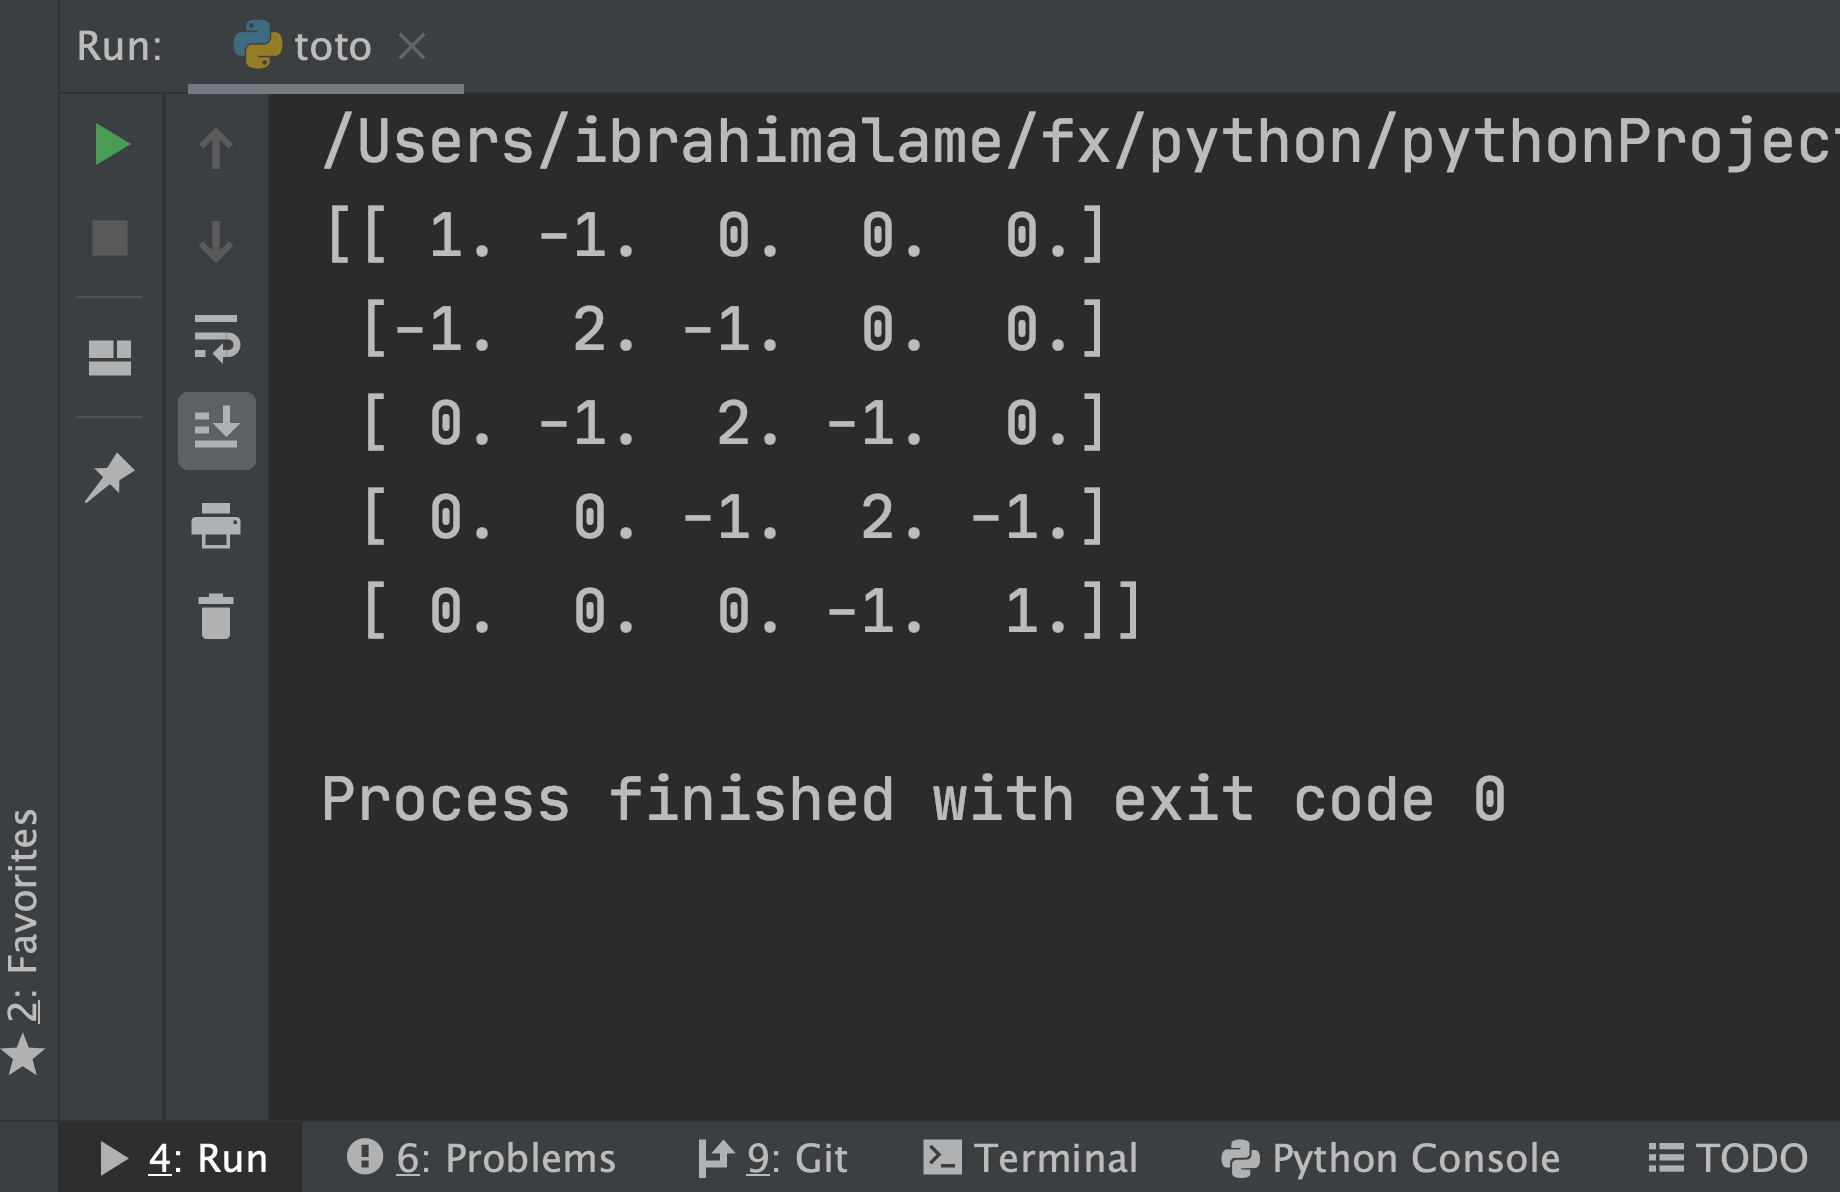
\includegraphics[scale=0.34]{codePython02.png} 
\end{center}

\end{frame}
%%%%%%%%%%%%%%%%%%%%%%%%%%%%%%%%%%%%%%%%%%%%%%%%%%%%%
%%%%%%%%%%%%%%%%%%%%%%%%%%%%%%%%%%%%%%%%%%%%%%%%%%%%%
\begin{frame}
\frametitle{Treillis soumis à une force nodale}
 trois poutres de même nature et de même section droite.
\begin{itemize}
\item Le noeud 1 est articulé et le nœud 3 repose sur un appui simple dont la normale est horizontale.
\item Le noeud 2 porte une charge de composantes (0, P ).
\end{itemize}
 \begin{center}
 \begin{tikzpicture}[scale=0.7]
\draw  [very thin, gray] [->]  (-2.5,0) -- (4,0); 
\draw  [very thin, gray] [->] (0,-6) -- (0,2);
\draw [double distance = 3pt] (0,0) -- (3,0) -- (0,-3*1.732) -- (0,0);
\path[fill=black]  (0,0) circle (2mm) [fill=gray];
\path[fill=black]  (3,0) circle (2mm) [fill=gray];
\path[fill=black]  (0,-3*1.732) circle (2mm) [fill=gray];
\draw [red,->,very thick] (3,0)-- (3,-2) node[right,midway]{$\vec{f_3}=\vec{P}$};
\draw [blue,->,very thick] (0,0)-- (-1.5,0) node[below,midway]{$\vec{f_0}$};
\draw [blue,->,very thick] (0,0)-- (0,1.5) node[right,midway]{$\vec{f_1}$};
\draw [blue,->,very thick] (0,-3*1.732)-- (1.2,-3*1.732) node[below,midway]{$\vec{f_4}$};
\draw (4,0) node[right] {$X$};
\draw (0,2) node[right] {$Y$};
%\draw [domain=0:5][line width=1] plot(\x,{.8598e-1*\x*\x*\x-.8104*\x*\x+1.697*\x});
%\draw [domain=0:6] plot(\x,{sin(57.29*\x)});
\end{tikzpicture} 

\end{center}


\end{frame}

%%%%%%%%%%%%%%%%%%%%%%%%%%%%%%%%%%%%%%%%%%%%%%%%%%%%%
\begin{frame}
\frametitle{Treillis soumis à une force nodale}
Le système élémentaire s'écrit:
\[\left(\begin{array}{r} 
f_{1}\\f_{2}
\end{array}\right)=\frac{1}{h}\left(\begin{array}{rr} 
1&-1\\-1&1
\end{array}\right) \left(\begin{array}{l} 
u_{1}\\u_{2}
\end{array}\right)
\]

\begin{center}
 \begin{tikzpicture}[scale=1]
\draw  [very thin, gray] [->]  (-0.2,0) -- (4,0); 
\draw  [very thin, gray] [->] (0,-0.2) -- (0,3);
\draw  [dashed] (1,0) -- (1,.5)--(0,.5);
\draw  [dashed] (3,0) -- (3,2.5)--(0,2.5);
\draw (1,0) node[below] {$X_i$};
\draw (3,0) node[below] {$X_j$};
\draw (-0.2,0.5) node[below] {$Y_i$};
\draw (-0.2,2.5) node[below] {$Y_j$};
\draw [double distance = 3pt] (1,0.5) -- (3,2.5);
\path[fill=black]  (1,.5) circle (1.2mm) [fill=gray];
\path[fill=black]  (3,2.5) circle (1.2mm) [fill=gray];
\coordinate (A) at (2,.5);
\draw[->,red] (A)  arc(0:45:1);
\draw[red] (2,.9) node[right]{$\theta$};
\draw  [dotted] (1,.5) -- (3,.5);
\draw  [very thin, gray] [->]  (0.8,0.3) -- (3.5,3.); 
\draw  [very thin, gray] [->] (1.2,0.3) -- (-1,2.5);
\draw (4,0) node[right] {$X$};
\draw (0,3.2) node[right] {$Y$};
\draw (3.5,3) node[right] {$x$};
\draw (-1,2.8) node[right] {$y$};
%\draw [domain=0:5][line width=1] plot(\x,{.8598e-1*\x*\x*\x-.8104*\x*\x+1.697*\x});
%\draw [domain=0:6] plot(\x,{sin(57.29*\x)});
\end{tikzpicture} 
\end{center}
\end{frame}

%%%%%%%%%%%%%%%%%%%%%%%%%%%%%%%%%%%%%%%%%%%%%%%%%%%%%
\begin{frame}
\frametitle{Formules de passage}
Les formules de passage entre les deux repères local $(x,y)$ et global $(X,Y)$:
\[\left(\begin{array}{l} 
u_{1}\\u_{2}
\end{array}\right) = \left(\begin{array}{cccc} 
\cos\theta &\sin\theta&0&0\\
0&0&\cos\theta &\sin\theta
\end{array}\right) \left(\begin{array}{l} 
U_{1}^x\\U_{1}^y\\U_{2}^x\\U_{2}^y
\end{array}\right)  \]
\[\left(\begin{array}{l} 
F_{1}^x\\F_{1}^y\\F_{2}^x\\F_{2}^y
\end{array}\right)   = \left(\begin{array}{cc} 
\cos\theta &0\\
\sin\theta& 0\\
0&\cos\theta \\
0 &\sin\theta
\end{array}\right)  \left(\begin{array}{l} 
f_{1}\\f_{2}
\end{array}\right)  \]


\end{frame}

%%%%%%%%%%%%%%%%%%%%%%%%%%%%%%%%%%%%%%%%%%%%%%%%%%%%%
\begin{frame}
\frametitle{Matrice de rigidité élémentaire dans le repère global}
\[\left(\begin{array}{l} 
F_{1}^x\\F_{1}^y\\F_{2}^x\\F_{2}^y
\end{array}\right)   = \frac{1}{L}\left(\begin{array}{rrrr} 
C^2&CS&-C^2&-CS\\
CS&S^2&-CS&-S^2\\
-C^2&-CS&C^2&CS\\
-CS&-S^2&CS&S^2
\end{array}\right)\left(\begin{array}{l} 
U_{1}^x\\U_{1}^y\\U_{2}^x\\U_{2}^y
\end{array}\right)  \]
Changement de notations !
\[\left(\begin{array}{l} 
f_{1}\\f_{2}\\f_{3}\\f_{4}
\end{array}\right)   = \frac{EA}{L}\left(\begin{array}{rrrr} 
C^2&CS&-C^2&-CS\\
CS&S^2&-CS&-S^2\\
-C^2&-CS&C^2&CS\\
-CS&-S^2&CS&S^2
\end{array}\right)\left(\begin{array}{l} 
\delta_{1}\\\delta_{2}\\\delta_{3}\\\delta_{4}
\end{array}\right)  \]
\end{frame}

%%%%%%%%%%%%%%%%%%%%%%%%%%%%%%%%%%%%%%%%%%%%%%%%%%%%%
\begin{frame}
\frametitle{Nœuds et connectivité}
Les caractéristique géométriques du système se résume en:\\
\begin{center}
\begin{tabular}{|l|c|r|}
  \hline
  nœud & $x$  & $y$ \\
  \hline
  0 & 0 & 0 \\
  1& $L$& 0 \\
  2& 0 & $-\sqrt 3 L$ \\
  \hline
\end{tabular} 
\end{center}

\begin{center}
  \begin{tabular}{|l|c|r|c|c|}
  \hline
  poutre & $\ell$  & $\theta$ & $C=\cos\theta$ & $S=\sin\theta$\\
  \hline
  (0,1) & $L$ & 0 & 1 & 0 \\
  (1,2)& $2L$& $-\frac{2\pi}{3}$&$-1/2$&$-\sqrt 3/2 $\\
  (2,0)& $\sqrt 3L$ &$\frac{\pi}{2}$ &0 &1 \\
  \hline
\end{tabular}
\end{center}

\end{frame}
%%%%%%%%%%%%%%%%%%%%%%%%%%%%%%%%%%%%%%%%%%%%%%%%%%%%%
\begin{frame}[fragile]
\frametitle{Matrice élémentaire de la barre (0,1):}
\[ \frac{EA}{L}\left(\begin{array}{rrrr} 
1&0&-1&0\\
0&0&0&0\\
-1&0&1&0\\
0&0&0&0
\end{array}\right)\]
La connectivité est définie par $n:(q,r)\mapsto [2q,2q+1,2r,2r+1]$ donc $n(0,1)=[0,1,2,3]$
\[
M =
\begin{tikzpicture}[baseline={([yshift=-\dimexpr\fontdimen22\textfont2\relax]M.center)}]
  \matrix [
    matrix of math nodes,
    left delimiter={[}, right delimiter={]},
    inner sep=1pt, column sep=1ex, row sep=1ex,
    execute at begin cell=\mathstrut,
  ] (M) {
    1 & 0 & -1 &  0  &  0 & 0\\
    0 &  0  & 0 & 0 & 0 & 0\\
    -1  &  0  &  1  & 0 &  0  & 0\\
    0  & 0 & 0 &  0  & 0 & 0\\
    0  & 0 &  0  & 0 & 0 & 0\\
    0  & 0 &  0  & 0 & 0 & 0\\
  };

	\node[above=1em,orange] at (M-1-1) {$\scriptstyle 0$};
    \node[above=1em,orange] at (M-1-2) {$\scriptstyle 1$};
    \node[above=1em,orange] at (M-1-3) {$\scriptstyle 2$};
    \node[above=1em,orange] at (M-1-4) {$\scriptstyle 3$};
  
    \node[left=1.5em,orange] at (M-1-1) {$\scriptstyle 0$};
    \node[left=1.5em,orange] at (M-2-1) {$\scriptstyle 1$};
    \node[left=1.5em,orange] at (M-3-1) {$\scriptstyle 2$};
    \node[left=1.5em,orange] at (M-4-1) {$\scriptstyle 3$};

\end{tikzpicture}
\]
\end{frame}

%%%%%%%%%%%%%%%%%%%%%%%%%%%%%%%%%%%%%%%%%%%%%%%%%%%%%
%%%%%%%%%%%%%%%%%%%%%%%%%%%%%%%%%%%%%%%%%%%%%%%%%%%%%
\begin{frame}[fragile]
\frametitle{Matrice élémentaire de la barre (1,2):}
\[
\frac{EA}{8L}\left(\begin{array}{rrrr} 
1&\sqrt 3&-1&-\sqrt 3\\
\sqrt 3&3&-\sqrt 3&-3\\
-1&-\sqrt 3&1&\sqrt 3\\
-\sqrt 3&-3&\sqrt 3&3\\
\end{array}\right)\]

La connectivité de l'élément $(1,2)$ est définie par la liste $n(1,2)=[2,3,4,5]$
\[
M =
\begin{tikzpicture}[baseline={([yshift=-\dimexpr\fontdimen22\textfont2\relax]M.center)}]
  \matrix [
    matrix of math nodes,
    left delimiter={[}, right delimiter={]},
    inner sep=1pt, column sep=1ex, row sep=1ex,
    execute at begin cell=\mathstrut,
  ] (M) {
  	0 & 0 & 0  & 0 &  0  & 0 \\
    0 & 0 & 0  & 0 &  0  & 0 \\
    0 & 0 & 1 & \sqrt 3 & -1 &  -\sqrt 3  \\
    0 & 0 &\sqrt 3 &  3  & -\sqrt 3 & -3 \\
    0  & 0 & -1  &  -\sqrt 3  &  1  & \sqrt 3 \\
    0 & 0 & -\sqrt 3  & -3 & \sqrt 3 &  3  \\
  };

	\node[above=1em,orange] at (M-1-3) {$\scriptstyle 0$};
    \node[above=1em,orange] at (M-1-4) {$\scriptstyle 1$};
    \node[above=1em,orange] at (M-1-5) {$\scriptstyle 2$};
    \node[above=1em,orange] at (M-1-6) {$\scriptstyle 3$};
  
    \node[left=2em,orange] at (M-3-1) {$\scriptstyle 0$};
    \node[left=2em,orange] at (M-4-1) {$\scriptstyle 1$};
    \node[left=2em,orange] at (M-5-1) {$\scriptstyle 2$};
    \node[left=2em,orange] at (M-6-1) {$\scriptstyle 3$};

\end{tikzpicture}\times\frac{EA}{8L}
\]


\end{frame}

%%%%%%%%%%%%%%%%%%%%%%%%%%%%%%%%%%%%%%%%%%%%%%%%%%%%%
%%%%%%%%%%%%%%%%%%%%%%%%%%%%%%%%%%%%%%%%%%%%%%%%%%%%%
\begin{frame}[fragile]
\frametitle{Matrice élémentaire de la barre (2,0):}
\[\frac{EA}{\sqrt 3L}\left(\begin{array}{rrrr} 
0&0&0&0\\
0&1&0&-1\\
0&0&0&0\\
0&-1&0&1
\end{array}\right)\]

La connectivité de l'élément $(2,0)$ est définie par la liste $n(2,0)=[4,5,0,1]$
\[
M =
\begin{tikzpicture}[baseline={([yshift=-\dimexpr\fontdimen22\textfont2\relax]M.center)}]
  \matrix [
    matrix of math nodes,
    left delimiter={[}, right delimiter={]},
    inner sep=1pt, column sep=1ex, row sep=1ex,
    execute at begin cell=\mathstrut,
  ] (M) {
    0 & 0 & 0 & 0  &  0 & 0\\
    0 &  1  & 0 & 0 & 0 & -1\\
    0  &  0  &  0  & 0 &  0  & 0\\
    0  & 0 & 0 &  0  & 0 & 0\\
    0  & 0 &  0  & 0 & 0 & 0\\
    0  & -1 &  0  & 0 & 0 & 1\\
  };

	\node[above=1em,orange] at (M-1-1) {$\scriptstyle 2$};
    \node[above=1em,orange] at (M-1-2) {$\scriptstyle 3$};
    \node[above=1em,orange] at (M-1-5) {$\scriptstyle 0$};
    \node[above=1em,orange] at (M-1-6) {$\scriptstyle 1$};
  
    \node[left=2em,orange] at (M-1-1) {$\scriptstyle 2$};
    \node[left=2em,orange] at (M-2-1) {$\scriptstyle 3$};
    \node[left=2em,orange] at (M-5-1) {$\scriptstyle 0$};
    \node[left=2em,orange] at (M-6-1) {$\scriptstyle 1$};

\end{tikzpicture}\times\frac{EA}{\sqrt 3L}
\]


\end{frame}

%%%%%%%%%%%%%%%%%%%%%%%%%%%%%%%%%%%%%%%%%%%%%%%%%%%%%

%%%%%%%%%%%%%%%%%%%%%%%%%%%%%%%%%%%%%%%%%%%%%%%%%%%%%
%%%%%%%%%%%%%%%%%%%%%%%%%%%%%%%%%%%%%%%%%%%%%%%%%%%%%
%%%%%%%%%%%%%%%%%%%%%%%%%%%%%%%%%%%%%%%%%%%%%%%%%%%%%
\begin{frame}
\frametitle{Matrice d'assemblage}
\[\left(\begin{array}{r}f_0\\ f_1\\f_2\\f_3\\f_4\\f_5 \end{array}\right) 
 =\frac{EA}{L}\left(\begin{array}{rrccrr} 
1&0&-1&0&0&0\\
0&\frac{1}{\sqrt 3}&0&0&0&-\frac{1}{\sqrt 3}\\
-1&0&1+\frac 18&\frac{\sqrt 3}{8}&-\frac 18&-\frac{\sqrt 3}{8}\\
0&0&\frac{\sqrt 3}{8}&\frac 38&-\frac{\sqrt 3}{8}&-\frac 38\\
0&0&-\frac 18&-\frac{\sqrt 3}{8}&\frac 18&\frac{\sqrt 3}{8}\\
0&-\frac{1}{\sqrt 3}&-\frac{\sqrt 3}{8}&-\frac 38&\frac{\sqrt 3}{8}&\frac{ 3}{8}+\frac{1}{\sqrt 3}
\end{array}\right)
\times
\left(\begin{array}{l}  \delta_0=0\\ u_1=0\\ u_2\\ u_3\\ u_4=0\\ u_5   \end{array}\right)
\]
Les trois déplacements nuls $u_0=u_1=u_4=0$ nous permettent de réduire le système et de supprimer de la matrice globale les trois lignes 0,1,4 et les trois colonnes 0,1,4. D'où le système linéaire:

\[\myredbox{
\left(\begin{array}{r} 0\\P\\0 \end{array}\right) 
=
\frac{EA}{L}\left(\begin{array}{rrr} 
1+\frac 18&\frac{\sqrt 3}{8}&-\frac{\sqrt 3}{8}\\
\frac{\sqrt 3}{8}&\frac 38&-\frac 38\\
-\frac{\sqrt 3}{8}&-\frac 38&\frac{ 3}{8}+\frac{1}{\sqrt 3}
\end{array}\right)
\times
\left(\begin{array}{r}   u_2\\ u_3\\ u_5  \end{array}\right) }
\]
\end{frame}

%%%%%%%%%%%%%%%%%%%%%%%%%%%%%%%%%%%%%%%%%%%%%%%%%%%%%
\begin{frame}
\frametitle{Résolution du système}
Après avoir résolu le système linéaire réduit, on reprend les équations éliminées du système globale pour déterminer les réactions aux appuis:
\[\begin{array}{l}
f_0=-\frac{EA}{L}u_2\\
f_1=-\frac{EA}{L}\frac{1}{\sqrt 3}u_5\\
f_4=\frac{EA}{L}\left(-\frac{\sqrt 3}{8} u_2-\frac{ 3}{8}u_3  +(\frac{ 3}{8}+\frac{1}{\sqrt 3})u_5\right)
\end{array}
\]
 On trouve $u_2\simeq 0.06$mm,  $u_3\simeq-0.47$mm,  $u_5\simeq-0.17$mm.\\
 et $f_0\simeq -5.8\times 10^3$N,  $f_1\simeq 1.0\times 10^4$N, $f_4\simeq 5.8\times 10^3$N.
 \begin{center}
 \begin{tikzpicture}[scale=0.6]
\draw  [very thin, gray] [->]  (-1,0) -- (4,0); 
\draw  [very thin, gray] [->] (0,-6) -- (0,0.5);
\draw [double distance = 3pt] (0,0) -- (3,0) -- (0,-3*1.732) -- (0,0);
\draw [blue,double distance = 3pt] (0,0) -- (3.06,-0.47) -- (0,-3*1.732-0.17) -- (0,0);
\draw [red,->,very thick] (3.06,-0.47)-- (3.06,-0.47-2);
\path[fill=black]  (0,0) circle (2mm) [fill=gray];
\path[fill=black]  (3,0) circle (2mm) [fill=gray];
\path[fill=black]  (0,-3*1.732) circle (2mm) [fill=gray];
\path[blue,fill=black]  (3.06,-0.47) circle (2mm) [fill=blue];
\path[blue,fill=black]  (0,-3*1.732-0.17) circle (2mm) [fill=blue];

\draw (4,0) node[right] {$X$};
\draw (0,0.5) node[right] {$Y$};
%\draw [domain=0:5][line width=1] plot(\x,{.8598e-1*\x*\x*\x-.8104*\x*\x+1.697*\x});
%\draw [domain=0:6] plot(\x,{sin(57.29*\x)});
\end{tikzpicture} 

\end{center}


\end{frame}

%%%%%%%%%%%%%%%%%%%%%%%%%%%%%%%%%%%%%%%%%%%%%%%%%%%%%
\begin{frame}[fragile]
\frametitle{Mise en œuvre numérique}

{\large Géométrie du problème}

\[Points=\left([x_i,y_i]\right)_{i=0,n-1}\]
\[Barres=\left([p_i,p_j]\right)_{(i,j)\in G}\]
 En python $N$ et $B$ sont codés par les deux listes suivantes:
\begin{verbatim}
L = .7
Points = [[0, 0], [0, L], [L, 0]]
Barres = [[0, 1], [1, 2], [2, 0]]
\end{verbatim}
Un nœud peut être articulé en un point fixe qui empêche tout déplacement  $u_1=u_2=0$, ou un appui simple horizontal ($u_2=0$) ou vertical ($u_1=0$). On représente la fixation d'un nœud par un triplet $\left(p_i,\alpha_i,\beta_i\right)$ où $p_i$ est le point considéré, $\alpha_i$ est un boolean qui vaut 1 si le déplacement horizontal est libre, 0 sinon, et $\beta_i$ est un boolean qui vaut 1 si le déplacement vertical est libre, 0 sinon. Pour notre exemple:
\begin{verbatim}
Conditions = [[0,0,0],[2,0,1]]
\end{verbatim}
\end{frame}

%%%%%%%%%%%%%%%%%%%%%%%%%%%%%%%%%%%%%%%%%%%%%%%%%%%%%
\begin{frame}[fragile]
\frametitle{Mise en œuvre numérique}
{\Large Les constantes et grandeurs physiques}

La section des barres $A$ exprimée en $\mbox{m}^2$. Les longueurs des barres $L_i$ sont calculées à partir des coordonnées des points d'articulation et exprimées en mètre (m). Le module de Young $E$ est exprimé en Pascal (Pa) . Les forces extérieurs nodales sont exprimées en Newton (N).

Pour notre exemple nous avons:
$L=0.2$m, $A=100\mbox{m}^2$, $E=200000$MPa, et $P=-10000$N.
\begin{verbatim}
L = 0.2
A = 100 * 1E-6
E = 200000 * 1E6
P = -10000
\end{verbatim}
\end{frame}

%%%%%%%%%%%%%%%%%%%%%%%%%%%%%%%%%%%%%%%%%%%%%%%%%%%%%
\begin{frame}[fragile]
\frametitle{Indexation}
\subsubsection{Matrice de rigidité}
Soit $B_i=(p1,p2)$ une barre du système d'extrémités $p_1=(X_1,Y_1)$ et $p_2=(X_2,Y_2)$. On calcule $\ell$ la longueur de la barre, $c$ et $s$, le cosinus et le sinus de l'angle $\theta$ que fait  la barre avec l'axe $(OX)$ par:
\[c=\cos \theta = \frac{X_2-X_1}{\ell}\mbox{ et }s=\sin \theta = \frac{Y_2-Y_1}{\ell},\quad \ell=\sqrt{(X_2-X_1)^2+(Y_2-Y_1)^2} \]
Si on désigne par $CS$ la matrice ligne $\left(\begin{array}{cccc}
c &s&-c& -s
\end{array}\right)$, la matrice de rigidité n'est autre que 
\[\mbox{\textbf{K}}_i=\frac{E A}{\ell} CS\times CS^t\]


\begin{center}
 \begin{tikzpicture}[scale=1]
\draw  [very thin, gray] [->]  (-0.2,0) -- (7,0); 
\draw  [very thin, gray] [->] (0,-0.2) -- (0,3);
\draw [double distance = 1pt] (1,0.5) -- (2,2.5)--(3.5,2)--(4,1)--(5.5,2.7)--(6.5,2.5);
\draw[double distance = 1pt] plot[mark=ball,mark size=1mm] coordinates {(1,0.5) (2,2.5)(3.5,2)(4,1)(5.5,2.7)(6.5,2.5)};
\path[fill=black]  (1,.5) circle (.75mm) [fill=gray];
\path[fill=black]  (2,2.5) circle (.75mm) [fill=gray];
\path[fill=black]  (3.5,2) circle (.75mm) [fill=gray];
\path[fill=black]  (4,1) circle (.75mm) [fill=gray];
\path[fill=black]  (5.5,2.7) circle (.75mm) [fill=gray];
\path[fill=black]  (6.5,2.5) circle (.75mm) [fill=gray];
\draw[red] (1.2,.6) node[below] {$0$};
\draw (.6,.5) node[above]{$(u_0,u_1)$} ;
\draw[red] (2.1,2.4) node[below] {$1$};
\draw (2,2.5) node[above] {$(u_2,u_3)$};
\draw[red] (3.3,2)  node[below] {$2$};
\draw (3.5,2.1) node[above] {$(u_4,u_5)$};
\draw[red] (5.7,2.6) node[below] {$i$};
\draw (5.5,2.7) node[above] {$(u_{2i},u_{2i+1})$};
\draw (7,0) node[below] {$X$};
\draw (0,3.2) node[right] {$Y$};

%\draw [domain=0:5][line width=1] plot(\x,{.8598e-1*\x*\x*\x-.8104*\x*\x+1.697*\x});
%\draw [domain=0:6] plot(\x,{sin(57.29*\x)});
\end{tikzpicture} 

\end{center}
\end{frame}

%%%%%%%%%%%%%%%%%%%%%%%%%%%%%%%%%%%%%%%%%%%%%%%%%%%%%
\begin{frame}[fragile]
\frametitle{Indexation}
Les nœuds sont numérotés $0,1,2,\dots ,q,\dots,r,\dots n-1$, on désigne par $(u_{2q},u_{2q+1})$ le vecteur déplacement du nœud $q$. L'équation matricielle d'équilibre d'une barre $(q,r)$ s'écrit matriciellement  en dimension $2n$:

\[
\begin{bmatrix}
  \vdots\\
 \vdots\\
     f_{2q} \\
    f_{2q+1} \\
   \vdots\\
     \vdots\\
     f_{2r} \\
     f_{2r+1} \\
     \vdots
\end{bmatrix}
=\frac{E A}{\ell} 
\begin{bmatrix}
        & \vdots & \vdots & & \vdots& \vdots&  \\
        & \vdots & \vdots & & \vdots& \vdots&  \\
     \dots      & C^2 & CS & \dots & -C^2& -CS& \dots \\
    \dots       & CS & S^2& \dots & -CS& -S^2& \dots\\
        & \vdots & \vdots & & \vdots& \vdots&  \\
        & \vdots & \vdots & & \vdots& \vdots&  \\
     \dots      & -C^2 & -CS & \dots & C^2& CS& \dots\\
      \dots      & -CS & -S^2 & \dots & CS& S^2& \dots\\
        & \vdots & \vdots & & \vdots& \vdots&  \\

\end{bmatrix}
\times
\begin{bmatrix}
  \vdots\\
 \vdots\\
     u_{2q} \\
    u_{2q+1} \\
   \vdots\\
     \vdots\\
     u_{2r} \\
     u_{2r+1} \\
     \vdots\\
\end{bmatrix}
\]
Les autres coefficients manquant sont tous nuls. 

\end{frame}

%%%%%%%%%%%%%%%%%%%%%%%%%%%%%%%%%%%%%%%%%%%%%%%%%%%%%
\begin{frame}[fragile]
\frametitle{Matrice d'assemblage}
\begin{minted}[
mathescape,
framesep=2mm,
baselinestretch=1.2,
%fontsize=\footnotesize,
bgcolor=LightGray,
%linenos
]{python}
import math
import numpy as np

L=0.7
A=100*1E-6
E=20000*1E6
P=-10000
Points = [[0,0],[0,L],[L,0]]
Barres = [[0,1],[1,2],[2,0]]
Conditions = [[0,0,0],[2,0,1]]
def n(q,r):
    return [2*q,2*q+1,2*r,2*r+1]
\end{minted}
  \end{frame}

%%%%%%%%%%%%%%%%%%%%%%%%%%%%%%%%%%%%%%%%%%%%%%%%%%%%%
\begin{frame}[fragile]
%\frametitle{Matrice d'assemblage}
\begin{minted}[
mathescape,
framesep=2mm,
baselinestretch=1.2,
%fontsize=\footnotesize,
bgcolor=LightGray,
%linenos
]{python}
for q,r in Barres:
    x1,y1 = Points[q]
    x2, y2 = Points[r]
    ell = math.sqrt((x2-x1)**2+(y2-y1)**2)
    c=(x2-x1)/ell
    s=(y2-y1)/ell
    CS = np.mat([c,s,-c,-s],dtype=float)
    CSt= np.transpose(CS)
    m = np.dot(CSt,CS)*A*E/ell
    for i in range(4):
        I=n(q,r)[i]
        for j in range(4):
            J=n(q,r)[j]
            M[I,J]+=m[i,j]
print(M)
\end{minted}
\end{frame}

%%%%%%%%%%%%%%%%%%%%%%%%%%%%%%%%%%%%%%%%%%%%%%%%%%%%%
\begin{frame}[fragile]
\frametitle{Matrice d'assemblage}
Les conditions aux appuis impose un ou deux déplacements nuls. On retire donc du système matriciel  les lignes et colonnes correspondants, soit en python:

\begin{minted}[
mathescape,
framesep=2mm,
baselinestretch=1.2,
%fontsize=\footnotesize,
bgcolor=LightGray,
%linenos
]{python}
l = []
for q, a, b in Conditions:
    if a == 0:
        l.append(2 * q)
    if b == 0:
        l.append(2 * q + 1)
l.sort()
l.reverse()
for i in l:
    M = np.delete(M, i, axis=0)
    M = np.delete(M, i, axis=1)
\end{minted}


\end{frame}

%%%%%%%%%%%%%%%%%%%%%%%%%%%%%%%%%%%%%%%%%%%%%%%%%%%%%
\begin{frame}[fragile]
\frametitle{Exemple}

  
\begin{center}
\begin{tikzpicture}[scale=1]
\appui{0}{0}{.3};
\appui{0}{-2}{.3};
\draw[double distance = 1pt] (0,0) - - (2,0);
\draw[double distance = 1pt] (2,0) - - (4,0);
\draw[double distance = 1pt] (4,0) - - (6,0);
\draw[double distance = 1pt] (6,0) - - (4,-2);
\draw[double distance = 1pt] (4,-2) - - (2,-2);
\draw[double distance = 1pt] (2,-2) - - (0,-2);
\draw[double distance = 1pt] (4,0) - - (2,-2);
\draw[double distance = 1pt] (2,0) - - (0,-2);
\draw[double distance = 1pt] (2,0) - - (2,-2);
\draw[double distance = 1pt] (4,0) - - (4,-2);
\path[fill=black]  (0,0) circle (.75mm) [fill=gray];
\path[fill=black]  (2,0) circle (.75mm) [fill=gray];
\path[fill=black]  (4,0) circle (.75mm) [fill=gray];
\path[fill=black]  (6,0) circle (.75mm) [fill=gray];
\path[fill=black]  (4,-2) circle (.75mm) [fill=gray];
\path[fill=black]  (2,-2) circle (.75mm) [fill=gray];
\path[fill=black]  (0,-2) circle (.75mm) [fill=gray];

\draw[red,double distance = 1pt] (0.0,0.0) - - (2.0300000000000002,-0.07242640687119303);
\draw[red,double distance = 1pt] (2.0300000000000002,-0.07242640687119303) - - (4.045,-0.1898528137423861);
\draw[red,double distance = 1pt] (4.045,-0.1898528137423861) - - (6.045,-0.24985281374238621);
\draw[red,double distance = 1pt] (6.045,-0.24985281374238621) - - (3.985,-2.189852813742386);
\draw[red,double distance = 1pt] (3.985,-2.189852813742386) - - (1.9849999999999999,-2.087426406871193);
\draw[red,double distance = 1pt] (1.9849999999999999,-2.087426406871193) - - (0.0,-2.0);
\draw[red,double distance = 1pt] (4.045,-0.1898528137423861) - - (1.9849999999999999,-2.087426406871193);
\draw[red,double distance = 1pt] (2.0300000000000002,-0.07242640687119303) - - (0.0,-2.0);
\draw[red,double distance = 1pt] (2.0300000000000002,-0.07242640687119303) - - (1.9849999999999999,-2.087426406871193);
\draw[red,double distance = 1pt] (4.045,-0.1898528137423861) - - (3.985,-2.189852813742386);
\path[fill=black]  (0.0,0.0) circle (.75mm) [fill=gray];
\path[fill=black]  (2.0300000000000002,-0.07242640687119303) circle (.75mm) [fill=gray];
\path[fill=black]  (4.045,-0.1898528137423861) circle (.75mm) [fill=gray];
\path[fill=black]  (6.045,-0.24985281374238621) circle (.75mm) [fill=gray];
\path[fill=black]  (3.985,-2.189852813742386) circle (.75mm) [fill=gray];
\path[fill=black]  (1.9849999999999999,-2.087426406871193) circle (.75mm) [fill=gray];
\path[fill=black]  (0.0,-2.0) circle (.75mm) [fill=gray];
(6.045,-0.24985281374238621)
\draw [blue,->,very thick] (6.045,-0.25)-- (6.045,-2.25);
\end{tikzpicture}
\end{center}
\end{frame}

%%%%%%%%%%%%%%%%%%%%%%%%%%%%%%%%%%%%%%%%%%%%%%%%%%%
%%%%%%%%%%%%%%%%%%%%%%%%%%%%%%%%%%%%%%%%%%%%%%%%%%%

\begin{frame}
\frametitle{Éléments finis 2D}
%Considérons le problème suivant:
\[
({\cal P}_v)\;\left\{
\begin{array}{l}
\mbox{Trouver } u\in V \mbox{ vérifiant}\\
a(u,v)=\ell(v)\quad \forall v\in V
\end{array}
\right.
\]

où \[ a(u,v)=\displaystyle \int_{\Omega}\nabla u\cdot \nabla v \quad \mbox{ et }\quad \ell(v)=\displaystyle \int_{\Omega}f v  \]
%Maillage
\begin{center}
\begin{tikzpicture}[domain=0:5,scale=1]
 \pgfmathsetmacro{\alpha}{0.05}
  \pgfmathsetmacro{\a}{1.2}
  \pgfmathsetmacro{\N}{3}
  \draw[->] (0,0) -- (\N*\a+\a/2,0)  node[right] {$x$};
  \draw[->] (0,0) -- (0,\N*\a+\a/2) node[left] {$y$};

  \foreach \n in {0,1,...,\N}{
   \draw[blue,thick](\n*\a,0)-- ++(0,\N*\a);
    \draw[blue,thick](0,\n*\a)-- ++(\N*\a,0);
}
  \foreach \n in {0,1,...,\N}{
   \draw[blue,thick](\n*\a,0)-- (\N*\a,\N*\a-\n*\a);
    \draw[blue,thick](0,\n*\a)-- (\N*\a-\n*\a,\N*\a);
}
  \foreach \i in {0,1,...,\N}{
  		\foreach \j in {0,1,...,\N}{
  		\pgfmathsetmacro{\x}{int(\N*\j+\j+\i)}
   \draw[red,thick](\i*\a,\j*\a-\a/4) node{\x};
   }
}
\pgfmathsetmacro{\M}{int(\N-1)}
  \foreach \i in {0,1,...,\M}{
  		\foreach \j in {0,1,...,\M}{
  		\pgfmathsetmacro{\x}{int(\N*\j+\j+\i)}
  		\pgfmathsetmacro{\k}{int(2*\i+2*\j*\N)}
   \draw[gray,thick](\i*\a+\a/3,\j*\a+2*\a/3) node{(\k)};
   \pgfmathsetmacro{\k}{int(2*\i+1+2*\j*\N)}
   \draw[gray,thick](\i*\a+2*\a/3,\j*\a+\a/3) node{(\k)};
   }
}



\draw (1*\a,0)  node[below] {$\scriptstyle  i h$};
\draw (0,2*\a)  node[left] {$\scriptstyle  j h$};
%\draw[fill=orange!30, fill opacity=0.6] (1*\a,2*\a)  -- ++(\a,0) -- ++(0,\a) ;
%  \path[fill=gray] (1*\a,2*\a) circle (0.6mm)node[left,below] {$\scriptstyle  a_{ij}$};
%  \draw[blue] (1.6*\a,2.2*\a) node{$\scriptstyle  K_{i,j,1}$};
%  \draw[fill=olive!30, fill opacity=0.6] (1*\a,2*\a)  -- ++(0,\a) -- ++(\a,0) ;
%  \draw[blue] (1.4*\a,2.8*\a) node{$\scriptstyle  K_{i,j,0}$};
\end{tikzpicture}
\end{center}


\end{frame}
%%%%%%%%%%%%%%%%%%%%%%%%%%%%%%%%%%%%%%%%%%%%%%%%%%%%%%%

\begin{frame}
\frametitle{Éléments finis triangles de type (1)}
\begin{center}
\begin{tikzpicture}[domain=0:5,scale=0.5]
 \pgfmathsetmacro{\alpha}{0.05}
  \pgfmathsetmacro{\a}{0.5}
  \draw[->] (0,0) -- (5,0)  node[right] {$\xi$};
  \draw[->] (0,0) -- (0,5) node[left] {$\eta$};
 \draw[->] (8,0) -- ++(7,0)  node[right] {$x$};
  \draw[->] (8,0) --++ (0,5) node[left] {$y$};
   \draw[blue,thick,fill=blue!30, fill opacity=0.6](10,2)-- ++(3,-1)-- ++(0,3)-- ++(-3,-2);

\path[fill=gray] (10,2) circle (1.0mm)node[left,below] {$\scriptstyle  C$};
\path[fill=gray] (13,1) circle (1.0mm)node[left,below] {$\scriptstyle  A$};
\path[fill=gray] (13,4) circle (1.0mm)node[right] {$\scriptstyle  B$};


\draw[fill=orange!30, fill opacity=0.6] (0,0) -- ++(3,0) -- ++(-3,3) -- ++(0,-3) ;
\path[fill=gray] (0,0) circle (1.0mm)node[left,] {$\scriptstyle \widehat{C} $};
\path[fill=gray] (3,0) circle (1.0mm)node[right,above] {$\scriptstyle  \widehat{A}$};
\path[fill=gray] (0,3) circle (1.0mm)node[left] {$\scriptstyle  \widehat{B}$};
\draw (2,0)  node[below] {$\scriptstyle  \widehat{x} =(\xi,\eta)$};
\draw (11,0)  node[below] {\small {\bf x} $\scriptstyle =\,(x,y)$};
  
 \draw [->, >=latex,olive] (1,1.5) arc (120:70:13) ;
\end{tikzpicture}

\end{center}
Nous avons 
\[x=\xi A + \eta B + (1-\xi-\eta) C\]
Donc \[e_1=\frac{\partial x}{\partial \xi}=A-C=\overrightarrow{CA}\]
		\[e_2=\frac{\partial x}{\partial \eta}=B-C=\overrightarrow{CB}\]

\end{frame}


%%%%%%%%%%%%%%%%%%%%%%%%%%%%%%%%%%%%%%%%%%%%%%%%%%%%%%%
\begin{frame}		
		
Donc la matrice jacobienne $Jacobienne=mat(e_1,e_2)$:
\[Jacobienne=\;<\overrightarrow{CA} \; \overrightarrow{CB}>\;=\left(\begin{array}{cc}
x_1-x_3 & x_2-x_3 \\
y_1-y_3 & y_2-y_3 
\end{array}\right)\]
Le jacobien est
\[\det J=\det(\overrightarrow{CA} , \overrightarrow{CB})\;=\left|\begin{array}{cc}
x_1-x_3 & x_2-x_3 \\
y_1-y_3 & y_2-y_3 
\end{array}\right| =\|\overrightarrow{CA}\|\cdot\|\overrightarrow{CB}\|\sin\alpha\]
On a donc 
\[|\det J|=\|\overrightarrow{CA}\wedge \overrightarrow{CB} \|\]
Le tenseur symétrique est
\[(g_{ij})=\left(\begin{array}{cc}
e_1\cdot e_1 & e_1\cdot e_2 \\
e_2\cdot e_1& e_2\cdot e_2
\end{array}\right) =\left(\begin{array}{cc}
\|\overrightarrow{CA}\|^2   &\overrightarrow{CA}\cdot \overrightarrow{CB} \\
\overrightarrow{CA}\cdot \overrightarrow{CB} & \|\overrightarrow{CB}\|^2
\end{array}\right)=J^t\cdot J\]

\[(g^{ij})=\frac{1}{\|\overrightarrow{CA}\wedge \overrightarrow{CB} \|^2}\left(\begin{array}{cc}
\|\overrightarrow{CB}\|^2   &-\overrightarrow{CA}\cdot \overrightarrow{CB} \\
-\overrightarrow{CA}\cdot \overrightarrow{CB} & \|\overrightarrow{CA}\|^2
\end{array}\right)\]

\end{frame}


%%%%%%%%%%%%%%%%%%%%%%%%%%%%%%%%%%%%%%%%%%%%%%%%%%%%%%%
\begin{frame}
\frametitle{Matrice élémentaire}

Soit la formule de changement de variables
\[\int_{K_e}(\cdots) \de x\de y=\int_{\widehat{K}}(\cdots) \sqrt{|g|} \de \xi\de \eta\]

On a alors pour un élément fini triangle $T_e=ABC$ de type (1):
\[\myredbox{\int_{T_e}(\cdots) \de x\de y=\int_{\widehat{T}}(\cdots) \|\overrightarrow{CA}\wedge \overrightarrow{CB} \| \de \xi\de \eta}\]

Nous avons aussi, en posant $G=(g^{ij})$:
\[\displaystyle \int_{K_e}\nabla \varphi_i\cdot \nabla \varphi_j\;\de x\de y=\int_{\widehat{K}}\frac{1}{\sqrt{|g|} } g^{ij}\frac{\partial \widehat{\varphi_i}}{\partial \xi_i}\frac{\partial \widehat{\varphi_j}}{\partial \xi_j}\de \xi\de \eta=\int_{\widehat{K}}\frac{1}{|J|} \nabla \widehat{\varphi_i}^t G  \nabla \widehat{\varphi_j}\de \xi\de \eta\]
Donc
\[\myredbox{\displaystyle \int_{K_e}\nabla \varphi_i\cdot \nabla \varphi_j\;\de x\de y=\int_{\widehat{K}}
{\tiny
\frac{1}{\|\overrightarrow{CA}\wedge \overrightarrow{CB} \|} 
}
\nabla \widehat{\varphi_i}^t 
{\tiny
\left(\begin{array}{cc}
\|\overrightarrow{CB}\|^2   &-\overrightarrow{CA}\cdot \overrightarrow{CB} \\
-\overrightarrow{CA}\cdot \overrightarrow{CB} & \|\overrightarrow{CA}\|^2
\end{array}\right) 
}
\nabla \widehat{\varphi_j}\de \xi\de \eta}\]

\end{frame}

%%%%%%%%%%%%%%%%%%%%%%%%%%%%%%%%%%%%%%%%%%%%%%%%%%%%%%%
%%%%%%%%%%%%%%%%%%%%%%%%%%%%%%%%%%%%%%%%%%%%%%%%%%%%%%%
\begin{frame}
\frametitle{Cas particulier élément fini triangle isocèle de type (1) }

\begin{center}
\begin{tikzpicture}[domain=0:5,scale=0.4]
 \pgfmathsetmacro{\alpha}{0.05}
  \pgfmathsetmacro{\a}{0.5}
  \draw[->] (0,0) -- (5,0)  node[right] {$\xi$};
  \draw[->] (0,0) -- (0,5) node[left] {$\eta$};
 \draw[->] (8,0) -- ++(8,0)  node[right] {$x$};
  \draw[->] (8,0) --++ (0,7) node[left] {$y$};
   \draw[blue,thick,fill=blue!30, fill opacity=0.6](11,2)-- ++(2,0)-- ++(-2,2)-- ++(0,-2);
	\draw[blue,thick,](13,2)-- ++(2,0)-- ++(-2,2)-- ++(0,-2);
	\draw[blue,thick,](11,4)-- ++(2,0)-- ++(-2,2)-- ++(0,-2);
	\draw[blue,thick,](9,4)-- ++(2,0)-- ++(-2,2)-- ++(0,-2);
	\draw[blue,thick,](9,2)-- ++(2,0)-- ++(-2,2)-- ++(0,-2);
	\draw[blue,thick,](9,0)-- ++(2,0)-- ++(-2,2)-- ++(0,-2);
	\draw[blue,thick,](11,0)-- ++(2,0)-- ++(-2,2)-- ++(0,-2);
	\draw[blue,thick,](13,0)-- ++(2,0)-- ++(-2,2)-- ++(0,-2);
	\draw[blue,thick,](13,4)-- ++(2,0)-- ++(-2,2)-- ++(0,-2);
	%\draw[blue,thick,](15,0)-- ++(0,2);
	\draw[blue,thick,](9,6)-- ++(6,0)--++(0,-6);
\path[fill=gray] (11,2) circle (1.0mm)node[below left] {$\scriptstyle  C$};
\path[fill=gray] (13,2) circle (1.0mm)node[below left] {$\scriptstyle  A$};
\path[fill=gray] (11,4) circle (1.0mm)node[above right] {$\scriptstyle  B$};


\draw[fill=orange!30, fill opacity=0.6] (0,0) -- ++(3,0) -- ++(-3,3) -- ++(0,-3) ;
\path[fill=gray] (0,0) circle (1.0mm)node[left,] {$\scriptstyle \widehat{C} $};
\path[fill=gray] (3,0) circle (1.0mm)node[right,above] {$\scriptstyle  \widehat{A}$};
\path[fill=gray] (0,3) circle (1.0mm)node[left] {$\scriptstyle  \widehat{B}$};
\draw (2,0)  node[below] {$\scriptstyle  \widehat{x} =(\xi,\eta)$};
\draw (11,0)  node[below] {\small {\bf x} $\scriptstyle =\,(x,y)$};
  
 \draw [->, >=latex,olive] (1,1.5) arc (120:70:13) ;
\end{tikzpicture}

\end{center}
\[\myredbox{a(\varphi_i,\varphi_j)=\displaystyle \int_{K_e}\nabla \varphi_i\cdot \nabla \varphi_j\;\de x\de y=\int_{\widehat{K}}
\nabla \widehat{\varphi_i}\cdot
\nabla \widehat{\varphi_j}\de \xi\de \eta}\]

\[\myredbox{\ell(\varphi_i)=\int_{T_e}f(x,y)\varphi_i(x,y) \de x\de y=h^2 \int_{\widehat{T}}\hat{f}(\xi,\eta)\widehat{\varphi_i}(\xi,\eta) \de \xi\de \eta}\]

\end{frame}
%%%%%%%%%%%%%%%%%%%%%%%%%%%%%%%%%%%%%%%%%%%%%%%%%%%%%%%
%%%%%%%%%%%%%%%%%%%%%%%%%%%%%%%%%%%%%%%%%%%%%%%%%%%%%%%

\begin{frame}
\frametitle{Éléments finis carré de type (1)}
\begin{center}
\begin{tikzpicture}[domain=0:5,scale=0.5]
 \pgfmathsetmacro{\alpha}{0.05}
  \pgfmathsetmacro{\a}{0.5}
  \draw[->] (0,0) -- (5,0)  node[right] {$\xi$};
  \draw[->] (0,0) -- (0,5) node[left] {$\eta$};
 \draw[->] (8,0) -- ++(7,0)  node[right] {$x$};
  \draw[->] (8,0) --++ (0,5) node[left] {$y$};
   \draw[blue,thick,fill=blue!30, fill opacity=0.6](10,2)-- ++(3,-1)-- ++(1,3)-- ++(-3,0)--++(-1,-2);

\path[fill=gray] (10,2) circle (1.0mm)node[left,below] {$\scriptstyle  A$};
\path[fill=gray] (13,1) circle (1.0mm)node[left,below] {$\scriptstyle  B$};
\path[fill=gray] (14,4) circle (1.0mm)node[right] {$\scriptstyle  C$};
\path[fill=gray] (11,4) circle (1.0mm)node[above left] {$\scriptstyle  D$};
 \draw[red,thick,->](11.8,2.8)-- ++(2.5,-0.3)node[right] {$\scriptstyle  e_1$};
  \draw[red,thick,->](11.8,2.8)-- ++(0.8,2.3)node[right] {$\scriptstyle  e_2$};

\draw[fill=orange!30, fill opacity=0.6] (0,0) -- ++(3,0)-- ++(0,3) -- ++(-3,0) -- ++(0,-3) ;
\path[fill=gray] (0,0) circle (1.0mm)node[left,] {$\scriptstyle \widehat{A} $};
\path[fill=gray] (3,0) circle (1.0mm)node[above right] {$\scriptstyle  \widehat{B}$};
\path[fill=gray] (3,3) circle (1.0mm)node[above right] {$\scriptstyle  \widehat{C}$};
\path[fill=gray] (0,3) circle (1.0mm)node[above left] {$\scriptstyle  \widehat{D}$};
\draw (2,0)  node[below] {$\scriptstyle  \widehat{x} =(\xi,\eta)$};
\draw (11,0)  node[below] {\small {\bf x} $\scriptstyle =\,(x,y)$};
  
 \draw [->, >=latex,olive] (1,1.5) arc (120:70:13) ;
\end{tikzpicture}

\end{center}
Nous avons 
\[x=\widehat{x}_3\widehat{x}_4 A + \widehat{x}_4\widehat{x}_1 B + \widehat{x}_1\widehat{x}_2 C +\widehat{x}_2\widehat{x}_3 D\]
\[x=(1-\xi)(1-\eta) A + (1-\eta)\xi B + \xi\eta C +(1-\xi)\eta D\]
Donc \[e_1=\frac{\partial x}{\partial \xi}=-(1-\eta) A+(1-\eta) B+\eta C-\eta D=(1-\eta)\overrightarrow{AB}+\eta\overrightarrow{DC}\]
		\[e_2=\frac{\partial x}{\partial \eta}=-(1-\xi) A-\xi B+\xi C+(1-\xi) D=(1-\xi)\overrightarrow{AD}+\xi\overrightarrow{BC}\]

\end{frame}


%%%%%%%%%%%%%%%%%%%%%%%%%%%%%%%%%%%%%%%%%%%%%%%%%%%%%%%
%%%%%%%%%%%%%%%%%%%%%%%%%%%%%%%%%%%%%%%%%%%%%%%%%%%%%%%
\begin{frame}		
		
Donc la matrice jacobienne $Jacobienne=mat(e_1,e_2)$:
\[Jacobienne=\;mat((1-\eta)\overrightarrow{AB}+\eta\overrightarrow{DC}, (1-\xi)\overrightarrow{AD}+\xi\overrightarrow{BC})\]
Le jacobien est
\[\det J=\det((1-\eta)\overrightarrow{AB}+\eta\overrightarrow{DC}, (1-\xi)\overrightarrow{AD}+\xi\overrightarrow{BC})\]

\[\begin{array}{lll}
\det J &= & (1-\eta)(1-\xi)\det(\overrightarrow{AB},\overrightarrow{AD})+(1-\eta)\xi\det(\overrightarrow{AB},\overrightarrow{BC})\\   
&  & +\eta (1-\xi)\det(\overrightarrow{DC},\overrightarrow{AD})+\eta \xi\det(\overrightarrow{DC},\overrightarrow{BC})
\end{array} \]
On a donc 
\[\myredbox{\det J=\det(\overrightarrow{AB},\overrightarrow{AD}) +\xi\det(\overrightarrow{AB},\overrightarrow{DC})+\eta \det(\overrightarrow{BC},\overrightarrow{AD})}\]

Le tenseur symétrique $(g_{ij})$ est
{\footnotesize
\[\left[\begin{array}{cc}
\|(1-\eta)\overrightarrow{AB}+\eta\overrightarrow{DC}\|^2   &\left[(1-\eta)\overrightarrow{AB}+\eta\overrightarrow{DC}\right]\cdot \left[(1-\xi)\overrightarrow{AD}+\xi\overrightarrow{BC}\right] \\
\left[(1-\eta)\overrightarrow{AB}+\eta\overrightarrow{DC}\right]\cdot \left[(1-\xi)\overrightarrow{AD}+\xi\overrightarrow{BC}\right] & \|(1-\xi)\overrightarrow{AD}+\xi\overrightarrow{BC}\|^2
\end{array}\right]\]
}
{\tiny
\[\myredbox{(g^{ij})=\frac{1}{\left(\det J\right)^2}\left[\begin{array}{cc}
\|(1-\xi)\overrightarrow{AD}+\xi\overrightarrow{BC}\|^2   &-\left[(1-\eta)\overrightarrow{AB}+\eta\overrightarrow{DC}\right]\cdot \left[(1-\xi)\overrightarrow{AD}+\xi\overrightarrow{BC}\right] \\
-\left[(1-\eta)\overrightarrow{AB}+\eta\overrightarrow{DC}\right]\cdot \left[(1-\xi)\overrightarrow{AD}+\xi\overrightarrow{BC}\right] & \|(1-\eta)\overrightarrow{AB}+\eta\overrightarrow{DC}\|^2 
\end{array}\right]}\]
}

\end{frame}


%%%%%%%%%%%%%%%%%%%%%%%%%%%%%%%%%%%%%%%%%%%%%%%%%%%%%%%
\begin{frame}
\frametitle{Cas particulier d'un élément fini parallélogramme}
\begin{center}
\begin{tikzpicture}[domain=0:5,scale=0.5]
 \pgfmathsetmacro{\alpha}{0.05}
  \pgfmathsetmacro{\a}{0.5}
  \draw[->] (0,0) -- (5,0)  node[right] {$\xi$};
  \draw[->] (0,0) -- (0,5) node[left] {$\eta$};
 \draw[->] (8,0) -- ++(7,0)  node[right] {$x$};
  \draw[->] (8,0) --++ (0,5) node[left] {$y$};
  
 \draw[fill=orange!30, fill opacity=0.6] (0,0) -- ++(3,0)-- ++(0,3) -- ++(-3,0) -- ++(0,-3) ;
\path[fill=gray] (0,0) circle (1.0mm)node[left,] {$\scriptstyle \widehat{A} $};
\path[fill=gray] (3,0) circle (1.0mm)node[above right] {$\scriptstyle  \widehat{B}$};
\path[fill=gray] (3,3) circle (1.0mm)node[above right] {$\scriptstyle  \widehat{C}$};
\path[fill=gray] (0,3) circle (1.0mm)node[above left] {$\scriptstyle  \widehat{D}$};
\draw (2,0)  node[below] {$\scriptstyle  \widehat{x} =(\xi,\eta)$}; 

  \draw[blue,thick](9,0)-- ++(1,4); 
  \draw[blue,thick](10,0)-- ++(1,4); 
    \draw[blue,thick](11,0)-- ++(1,4); 
      \draw[blue,thick](12,0)-- ++(1,4); 
        \draw[blue,thick](13,0)-- ++(1,4); 
        \draw[blue,thick](4/4+8,0)-- ++(4,0);
    \draw[blue,thick](5/4+8,1)-- ++(4,0);
    \draw[blue,thick](6/4+8,2)-- ++(4,0);     
        \draw[blue,thick](7/4+8,3)-- ++(4,0);         
        \draw[blue,thick](8/4+8,4)-- ++(4,0);               
   \draw[blue,thick,fill=blue!30, fill opacity=0.6](11.5,2)-- ++(1,0)-- ++(0.25,1)-- ++(-1,0)--++(-0.25,-1);

\path[fill=gray] (11.5,2) circle (1.0mm)node[below left] {\tiny  A};
\path[fill=gray] (12.5,2) circle (1.0mm)node[below right] {\tiny  B};
\path[fill=gray] (12.75,3) circle (1.0mm)node[above right] {\tiny  C};
\path[fill=gray] (11.75,3) circle (1.0mm)node[above left] {\tiny  D};


\draw (11,0)  node[below] {\small {\bf x} $\scriptstyle =\,(x,y)$};
  
 \draw [->, >=latex,olive] (1,1.5) arc (120:70:13.2) ;
\end{tikzpicture}
\end{center}
\[\myredbox{\det J=\det(\overrightarrow{AB},\overrightarrow{AD})}\]
\[(g_{ij}) =\left(\begin{array}{cc}
\|\overrightarrow{AB}\|^2   &\overrightarrow{AB}\cdot \overrightarrow{AD} \\
\overrightarrow{AB}\cdot \overrightarrow{AD} & \|\overrightarrow{AD}\|^2
\end{array}\right)\]
\[\myredbox{(g^{ij})=\frac{1}{\|\overrightarrow{AB}\wedge \overrightarrow{AD} \|^2}\left(\begin{array}{cc}
\|\overrightarrow{AD}\|^2   &-\overrightarrow{AB}\cdot \overrightarrow{AD} \\
-\overrightarrow{AB}\cdot \overrightarrow{AD} & \|\overrightarrow{AB}\|^2
\end{array}\right)}\]



\end{frame}
%%%%%%%%%%%%%%%%%%%%%%%%%%%%%%%%%%%%%%%%%%%%%%%%%%%%%%%
\begin{frame}
\frametitle{Matrice élémentaire}
\begin{itemize}
\item Matrice $A=(a_{ij})_{1\leq i,j \leq 3}$ où 
\[a(\varphi_i,\varphi_j)=\displaystyle \iint_{\widehat{K}}\nabla \widehat{\varphi_i} \cdot \nabla \widehat{\varphi_j}\;\de\xi\de\eta\]
où
\[\widehat{\varphi_1}=\xi,\quad \widehat{\varphi_2}=\eta,\quad \widehat{\varphi_3}=1-\xi-\eta\] 
\[\nabla\widehat{\varphi_1}=\left(\begin{array}{c} 1\\0\end{array}\right)
 ,\quad \nabla\widehat{\varphi_2}=\left(\begin{array}{c} 0\\1\end{array}\right),\quad \nabla\widehat{\varphi_3}=\left(\begin{array}{c} -1\\-1\end{array}\right)\] 
 \[\myredbox{A=\frac 12 \left(\begin{array}{ccc} 1&0&-1\\0&1&-1\\-1&-1&2\end{array}\right)}\]
 \item Second membre $B=(b_i)_{1\leq i\leq 3}$ où
 \[\myredbox{b_{i} = \ell(\varphi_i)=\displaystyle \iint_{K_e} f \varphi_i \;\de x\de y =h^2\displaystyle \iint_{\widehat{K}} f \widehat{\varphi_i} \;\de\xi\de\eta}\] 
\end{itemize}
\end{frame}


%%%%%%%%%%%%%%%%%%%%%%%%%%%%%%%%%%%%%%%%%%%%%%%%%%%

\begin{frame}
\frametitle{Maillage}
\begin{itemize}
\item  Table de nœuds:
\begin{center}
\begin{tabular}{|c|c|c|c|c|c|c|c|c|c|c|c|c|c|c|c|c|c|}\hline 
{\bf n} & 0 & 1 & 2 & 3 &4 &5 &6 & 7 & 8 &9 &10 & 11  & 12 &13 &14 & 15\\ \hline 
$\mbox{\bf i} $& $0$ & $1$ & 2 & 3 & $0$ & $1$ & 2 & 3& $0$ & $1$ & 2 & 3& $0$ & $1$ & 2 & 3\\ \hline 
$\mbox{\bf j} $& $0$ & $0$ & 0 & 0 & 1 & $1$ & 1 & 1&2&2&2&2  &3&3&3&3\\ \hline 
\end{tabular}
\end{center}
\item Table de connectivité:
\begin{center}
\begin{tabular}{|c|c|c|c|c|c|c|c|c|c|c|c|c|c|c|c|c|}\hline 
{\bf e} & 0 & 1 & 2 & 3 & 4 & 5 & 6 & 7 & 8 &9  &10 & 11  & 12 &... & 17\\ \hline 
{\bf 0}& 0  & 5 & 1 & 6 & 2 & 7 & 4 & 9& 5 &10 & 6 & 11 & 8 & ... &  15\\ \hline 
{\bf 1}& 5 & 0  & 6 & 1 & 7 & 2 & 9 & 4&10&5  &11 &6   &13&... &10\\ \hline 
{\bf 2}& 4 & 1  & 5 & 2 & 6 & 3 & 8 & 5&9 &6  &10  &7   &12&... &11\\ \hline 
\end{tabular}
\end{center}
\end{itemize}




\end{frame}





\end{document}